我们在第一章里简要地提到,量子力学可用两种观点处理。
第一,薛定谔波动力学将本征值方程表示为一个或多个变量函数的微分方程形式。
为了建立讨论薛定谔波函数所需的那种语言,在第二章里我们深入地研究了正交函数概念。
我们用解这样的微分方程(勒让德微分方程),并将其解与已建立的正交归一函数概念和性质联系起来做为总结。

研究量子力学的第二种观点是海森堡矩阵力学。本章将要建立研究矩阵力学的代数词汇。
也要以较完整的方式介绍在第一章里已提到的算符,导出量子化学中某些传统的有趣和重要结果。

\section{绪言}
我们就开始介绍一连串定义。
\begin{definition}[n维向量]
    一$n$维向量是$n$个数排成的数组:$\alpha=(\alpha_1,\alpha_2, \cdots ,\alpha_n)$。这n个数$\alpha_1,\alpha_2, \cdots ,\alpha_n$叫做向量的分量;它们是按规定的顺序排列;它们可为实数或虚数。
 \end{definition}

我们用希腊字母表示向量。三维空间中习用的物理向量就是一例,它的$x,y,z$分量分别用三个数表示。
\begin{definition}[向量空间]
    定义向量空间是具有下列二性质的向量的集合:
    
    (a) 定义唯一可对易的向量和为$\alpha^1+\alpha^2=\alpha^2+\alpha^1=(\alpha^1_1+\alpha^2_1,\alpha^1_2+\alpha^2_2,\cdots,\alpha^1_n+\alpha^2_n)$。
    
    (b) 定义任一向量$\alpha$和任一标量$c$的唯一积为$c\alpha=(c\alpha_1,c\alpha_2,\cdots,\alpha+n$,它既遵守分配律[即$c(\alpha+\beta)=c\alpha+c\beta$]又遵守结合律[即$(c_1c_2)\alpha=c_1(c_2\alpha)$]。    
\end{definition}

同学们应了解三维物理向量的这些性质。我们用上标表示向量组的成员${\alpha^i}$,用下标表示单个向量的分量。
\begin{definition}[欧氏向量空间]
    欧氏向量空间是这样的向量空间,其向量的分量是实数的,且任二向量的内积$\bra*{\alpha}\ket*{\beta}=\alpha_1\beta_1+\alpha_2\beta_2+\cdots+\alpha_n\beta_n$是实数的,
    它是对称的[$\bra*{\alpha}\ket*{\beta}=\bra*{\beta}\ket*{\alpha}$],双线性的[$\bra*{\alpha+\beta}\ket*{\gamma}=\bra*{\alpha}\ket*{\gamma}+\bra*{\beta}\ket*{\gamma}$]
    \footnote{关于双线性的定义应该是$\bra*{c_1\alpha^1+c_2\alpha^2}\ket*{\beta}=c_1\bra*{\alpha^1}\ket*{\beta}+c_2\bra*{\alpha^2}\ket*{\beta},\bra*{\alpha}\ket*{c_1\beta^1+c_2\beta^2}=c_1\bra*{\alpha}\ket*{\beta^1}+c_2\bra*{\alpha}\ket*{\beta^2}$,下一个定义中的双线性也相同。},和正值的[$\bra*{\alpha}\ket*{\alpha} \geq 0$]。
\end{definition}

此内积定义用的符号$\bra*{}\ket*{}$就是函数内积用的符号。

在稍微不同和更一般化的向量空间定义中,内积的定义也稍微不同和更一般化。
\begin{definition}[厄米向量空间]
    厄米向量空间是这样的向量空间, 其向量的分量可为复数,且任二向量可有复数内积$\bra*{\alpha}\ket*{\beta}=\alpha_1^*\beta_1+\alpha_2^*\beta_2+\cdots+\alpha_n^*\beta_n$,
    它是厄米的[$\bra*{\alpha}\ket*{\beta}=\bra*{\beta}\ket*{\alpha}^*$],双线性的[$\bra*{\alpha+\beta}\ket*{\gamma}=\bra*{\alpha}\ket*{\gamma}+\bra*{\beta}\ket*{\gamma}$],和正值的[$\bra*{\alpha}\ket*{\alpha} \geq 0$]。    
\end{definition}

应做两个比较。首先,比较这里的内积定义
\[\bra*{\alpha}\ket*{\beta}=\sum_i\alpha^*_i\beta_i \tag{3-1}\]
和第二章里内积的定义(方程2-1)
\[\bra*{f}\ket*{g}=\int f^*(x)g(x)\dd{x}\]
其差别在于向量内积定义是对不连续指标求和,而函数内积则是对连续变量积分。
此差别(不连续指标替换连续变量)在辨别海森堡和薛定谔图象时更明显。

另外,应看到欧氏向量空间和厄米向量空间的区别:欧氏向量空间中内积是实的和对称的;厄米向量空间中内积是复的和厄米的。
应将厄米向量空间中内积的这个性质和二函数内积的类似性质忆比:内积换位给出该内积的复共轭。
\begin{definition}[向量正交]
    若二向量的内积为零,则此二向量正交。
\end{definition}

此定义与函数正交性的定义是严格平行的;这使正交性成为一个更广义的概念,并与垂直向量这一为人们熟悉的性质建立联系。
\begin{definition}[向量范数]
    同样与已讲过的函数的有关内容类比,向量的范数定义为:$N(\alpha)=\bra*{\alpha}\ket*{\alpha}=\abs*{\alpha}^2$。
\end{definition}

范数对应于三维物理向量空间中向量的长度。最后的两个定义继续表明向量空间代数与函数微积分的平行结构。

\begin{definition}[向量归一化,正交归一向量组]
    若一向量的范数为一,则称该向量是归一化的。
    
    若向量组中每一向量是归一化的,且任一向量与任一其它向量都正交,则该向量组是正交归一向量组。
\end{definition}

我们用证明施瓦兹不等式做为对这些定义的说明。

\begin{theorem}[施瓦兹不等式]
    \[\abs*{\bra*{\alpha}\ket*{\alpha}} \leq \abs*{\alpha} \cdot \abs*{\beta}\]
\end{theorem}

若$\alpha$或$\beta$为零,则为等号,但定理没有意义。若$\alpha$和$\beta$都不为零,则可借二任意标量$c$和$d$之助构成此定理。根据内积的正值性,
\[0 \leq \bra*{c\alpha+d\beta}\ket*{c\alpha+d\beta} \tag{3-2}\]
和内积的双线性关系
\[0 \leq c^*\bra*{\alpha}\ket*{c\alpha+d\beta}+d^*\bra*{\beta}\ket*{c\alpha+d\beta}\]
\[\leq c^*c\bra*{\alpha}\ket*{\alpha}+c^*d\bra*{\alpha}\ket*{\beta}+d^*c\bra*{\beta}\ket*{\alpha}+d^*d\bra*{\beta}\ket*{\beta} \tag{3-3}\]
c和d为任何值方程都成立;因此,对特定值$c=-\bra*{\alpha}\ket*{\beta}$和$d=\bra*{\alpha}\ket*{\alpha}$方程也应成立。将这些值代入方程3-3,得出
\[0 \leq c^*cd-c^*dc-d^*cc^*+d^*d\bra*{\beta}\ket*{\beta}=d^*[-cc^*+d\bra*{\beta}\ket*{\beta}] \tag{3-4}\]
因此,
\[0 \leq -\abs*{\bra*{\alpha}\ket*{\beta}}^2+\bra*{\alpha}\ket*{\alpha}\bra*{\beta}\ket*{\beta} \tag{3-5}\]
或
\[\abs*{\bra*{\alpha}\ket*{\beta}}^2 \leq \abs*{\alpha}^2\abs*{\beta}^2 \tag{3-6}\]
\[\abs*{\bra*{\alpha}\ket*{\beta}} \leq \abs*{\alpha}\abs*{\beta} \tag{3-7}\]

建立了对函数和向量都能应用的内积和范数的定义后,我们就可以将对函数已深入研究过的那些结果应用于向量。
先考虑向量组;其结果在很大程度上与早先研究函数组的结果平行。

向量空间有与函数组完备性类似的概念。
\begin{definition}[向量空间]
    若向量空间的任一向量都能用向量组$\{\alpha^i\}$的线性组合表示,则该向量空间为向量组$\{\alpha^i\}$张成(Span)。
\end{definition}

通常的三维欧氏向量空间(以后称之为3D空间)能够很容易地将此定义用图表示出来。
例如,向量$(1,0,0),(0,1,0),(0,0,1)$张成3D空间。
这些向量正是三个坐标方向上的单位向量,任何向量可用三单位向量的线性组合表示,这是大家熟悉的事实。
这个定义促使我们对维的概念做更严格的解释。

\begin{definition}[向量空间的维数]
    向量空间的维是张成该向量空间所需的向量的最小数目。
\end{definition}

在上例中任二向量都不足以张成3D空间,但四个向量,如$(1,0,0),(0,1,0),(0,0,1),(1,1,1)$,又是多余的。
向量组$(1,0,0),(0,1,0),(1,1,0)$虽然数目是三,但不能张成3D空间。
希望读者能看出为什么。这些向量不是线性无关的,因而有一个是多余的。这样,线性无关的概念又在讨论向量空间时出现。

\begin{definition}[线性相关,线性无关]
    若只有全部$c_i=0$时方程
    \[c_1\alpha^1+c_2\alpha^2+\cdots+c_n\alpha^n=\sum_ic_i\alpha^i=0 \tag{3-8}\]
    才可解,则向量组$c_1 ,c_2,\cdots,c_n$是线性无关的。若方程3-8在某些$c_i \neq 0$时可解,则向量组$\{\alpha^i\}$是线性相关的。
\end{definition}

向量空间的这些性质使我们得出基这一方便概念。

\begin{definition}[基,正交归一基]
    向量空间的基是可张成向量空间的某些线性无关的向量组;
    
    向量空间的正交归一基是可张成该空间的某些正交归一向量组。
\end{definition}

可将此定义与由线性无关函数组造正交归一函数组的过程(施密特正交化)联系起来。施密特正交化可不加修正地用于向量。
若用$\{\alpha^i\}$表示线性无关向量组,$\{\phi^i\}$表示正交归一向量组,则可得有关公式如下:
\[\phi^k=\frac{1}{\sqrt{N_k}}(\alpha^k-\sum_{j=0}^{k-1}\bra*{\phi^j}\ket*{\phi^k}\phi^j) \tag{3-9}\]
\[N_k=\bra*{\alpha^k}\ket*{\alpha^k}-\sum_{j=0}^{k-1}\abs*{\bra*{\phi^j}\ket*{\phi^k}}^2 \tag{3-10}\]

由于向量几乎在所有方面都与正交归一函数平行,无疑全部代数“机器”都可用于将向量展成正交归一向量组。
在第二章中放在一起的那组方程(方程2-19——2-24) 可精确地用于向量问题。
因此,可按下列公式将任一向量$\xi$展成向量组$\{\phi^i\}$
\[\xi=\sum_ic_i\phi^i \tag{3-11}\]
其展开系数(可能是复数)为
\[c_i=-\bra*{\phi^i}\ket*{\xi} \tag{3-12}\]

也可从第二章将内积的展开定理借来用,
\[\bra*{\xi}\ket*{\eta}=\sum_i\bra*{\xi}\ket*{\phi^i}\bra*{\phi^i}\ket*{\eta} \tag{3-13}\]
式中$\{\phi^i\}$是正交归一向量组。

离开平行研究向量空间和函数,讨论一有用问题 ,这就是对有限维向量空间直接检验向量组是否线性无关。
读者可能还记得,在讨论函数组时曾暂时离开主题谈到此问题,并且更多地依赖直觉而非严格推理。

然而,对向量组我们可以仔细地作分析以确定向量组(有限的)是否线性无关。
由于出现了称为矩阵的数学元素,故此分析既为本节作出适合的总结,又是下节的导言。
在考虑线性无关时,我们尝试求符合方程3-8而又不为零的$c_i$。为了使求法比尝试法好些,提出一简单步骤。

将向量排成行。设有三个向量$\alpha,\beta,\gamma$每个向量有四个分量。其排列的形状如下:
\[
\begin{array}{cccc}
    \alpha_1 & \alpha_2 & \alpha_2 & \alpha_2 \\
    \beta_1 & \beta_2 & \beta_3 & \beta_4 \\
    \gamma_1 & \gamma_2 & \gamma_3 & \gamma_4
\end{array}    
\]
从底行作起。一定能找到一倍数乘$\alpha_1$加$\gamma_1$等于零。事实上此倍数就是$-\frac{\gamma_1}{\alpha_1}$。
将第一行所有$\alpha_1$;都乘此常数并加到底行上。现在排列的形状如下:
\[
\begin{array}{llll}
    \alpha_1 & \alpha_2 & \alpha_2 & \alpha_2 \\
    \beta_1 & \beta_2 & \beta_3 & \beta_4 \\
    0 & \gamma_2-\frac{\gamma_1}{\alpha_1}\alpha_2 & \gamma_3-\frac{\gamma_1}{\alpha_1}\alpha_3 & \gamma_4-\frac{\gamma_1}{\alpha_1}\alpha_4
\end{array}    
\]
用同样方法可以“消去”$\beta_1$,即找出一倍数乘$\alpha_1$加$\beta_1$:等于零。继续进行下去(下一步是消去$\gamma_2$),可得出下边那样排列:
\[
\begin{array}{llll}
    \times & \times & \times & \times \\
    0 & \times & \times & \times \\
    0 & 0 & \times & \times
\end{array}    
\]
像这样没有一行全为零,而左下角全为零的排列表明$\alpha,\beta,\gamma$线性组合都不为零,因而这些向量是线性无关的。若排列形状如下:
\[
\begin{array}{llll}
    \times & \times & \times & \times \\
    0 & \times & \times & \times \\
    0 & 0 & 0 & 0
\end{array}    
\]
则有$\alpha,\beta,\gamma$的某些线性组合为零(底行),因而这些向量是线性相关的。

现在可将这种想法归纳成文。

\begin{definition}
    \textbf{矩阵} \quad 标量(实数或复数)的矩形排列叫做矩阵。位于第$i$行第$j$列的标量称为矩阵的$i,j$矩阵元。$n$行$m$列的矩阵记为$n \times m$矩阵。

    \textbf{矩阵初等运算} \quad 对矩阵实施的初等行运算为:

    1.用常数乘行。
    
    2.两行相加。
    
    3.交换两行。

    \textbf{对角元} \quad 矩阵A的对角线(或主对角线)上的矩阵元为$\{a_{ii}\}$,即$a_{11},a_{22},a_{33},\cdots$等等。这些矩阵元称为对角元。
    
    \textbf{三角矩阵} \quad 若一矩阵其对角左下方的矩阵元皆为零,则该矩阵称为三角矩阵。\footnote{这里更应该叫上三角矩阵。}

    \textbf{行等价} \quad 用初等行运算可彼此形成的矩阵称为行等价。

    \textbf{向量组的线性无关} \quad 若以向量的分量为行形成的矩阵是非\footnote{这里译作“无”更好。}全为零的行的三角矩阵的行等价矩阵,则此向量组是线性无关的。
\end{definition}

此定理表示\footnote{奇怪的表述方式,感觉“揭示”更好。}出我们提出的检验线性无关的方法。用二例说明该定理和方法。

\textbf{例1}

向量$(1,-1,3),(2,-4,1)(0,3,2)$线性无关吗?先形成矩阵(放在括号里),再进行初等行运算。
(3,1)矩阵元已经是零。-2乘第一行加到第二行上使(2,1)矩阵元为零。为了简化,用$-\frac{1}{2}$乘第二行。
-3乘第二行加到第三行,上使(3,2)矩阵元为零。现在矩阵成三角形。所有行都至少含一不为零的矩阵元;因此,这些向量是线性无关的。

\[
\begin{pmatrix}
    1 & -1 & 3 \\
    2 & -4 & 1 \\
    0 & 3 & 2
\end{pmatrix}    
\xrightarrow{r_2-2r_1}
\begin{pmatrix}
    1 & -1 & 3 \\
    0 & -2 & -5 \\
    0 & 3 & 2
\end{pmatrix} 
\xrightarrow{-\frac{1}{2} \cdot r_2}
\begin{pmatrix}
    1 & -1 & 3 \\
    0 & 1 & \frac{5}{2} \\
    0 & 3 & 2
\end{pmatrix} 
\xrightarrow{r_3-3r_2}
\begin{pmatrix}
    1 & -1 & 3 \\
    0 & 1 & \frac{5}{2} \\
    0 & 0 & -\frac{11}{2}
\end{pmatrix} 
\]

\textbf{例2}

向量$(1,2i,1+i),(4,6-i,7),(-2,-6+5i,-5+2i)$线性无关吗?
还是先形成矩阵,再系统地实 施初等行运算。
\[
\begin{pmatrix}
    1 & 2i & 1+i \\
    4 & 6-i & 7 \\
    -2 & -6+5i & -5+2i
\end{pmatrix}    
\xrightarrow{r_3+2r_1}
\begin{pmatrix}
    1 & 2i & 1+i \\
    4 & 6-i & 7 \\
    0 & -6+9i & -3+4i
\end{pmatrix}    
\xrightarrow{r_2-3r_1}
\begin{pmatrix}
    1 & 2i & 1+i \\
    0 & 6-9i & 3-4i \\
    0 & -6+9i & -3+4i
\end{pmatrix}
\]
\[
\xrightarrow{r_3+r_2}
\begin{pmatrix}
    1 & 2i & 1+i \\
    0 & 6-9i & 3-4i \\
    0 & 0 & 0
\end{pmatrix}
\]

矩阵成三角形。有一行全为零;因此,这些向量线性相关。我们能够返回来作并求出满足方程3-8的常数:
\[2\alpha^1+\alpha^3+(-4\alpha^1+\alpha^2)=0\]
\[-2\alpha^1+\alpha^2+\alpha^3=0\]

本节用与函数对比的方法导出向量的-些性质。施密特正交化,展成正交归-基组,展开定理都是从第二章借来的结果。
介绍了检验线性无关的简易方法。在此检验方法中引入称为矩阵的代数元素,以及它的某些性质和成分,诸如矩阵元,对角元,行和列,行等价。

\section{矩阵、行列式和线性方程组}
矩阵。在上节中矩阵的定义是做为检验向量的线性无关的形式辅助手段而引入的。而矩阵有比做为这种问题的辅助手段更多的用途。
从量子力学的观点看,如第一章已提出的那样,矩阵可用来表示算符。矩阵的这个用途将在本章第四节详细讨论,它也促使我们现在要讨论更多的矩阵性质。

\begin{definition}[矩阵加法]
    二矩阵只有维数相同才能相加。$n \times m$矩阵A与$n \times m$矩阵B的和是$n \times m$矩阵C,其矩阵元由下列给出:
    \[c_{ij}=a_{ij}+b_{ij} \tag{3-14}\]
\end{definition}

也就是说,矩阵相加就是它们的矩阵元相加。我们用大写字母记矩阵,小写字母记它们的矩阵元。

\textbf{例}
\[
\begin{pmatrix}
    1 & 3 & 2 & 5 \\
    0 & 7 & 9 & 4 \\
    6 & -2 & 5 & 1 
\end{pmatrix}    
+
\begin{pmatrix}
    4 & -3 & 1 & -6 \\
    0 & 0 & -2 & 1 \\
    1 & -1 & 1 & -1 
\end{pmatrix}
=
\begin{pmatrix}
    5 & 0 & 3 & -1 \\
    0 & 7 & 7 & 5 \\
    7 & -3 & 6 & 0 
\end{pmatrix}   
\]

相加的定义不会使同学们惊异,而相乘的定义却与二数相显的通常概念不同。

\begin{definition}[矩阵乘法]
    只有乘数矩阵的列与被乘矩阵的行相同时,二矩阵才可相乘。$n \times m$矩阵4与$m \times p$矩阵B相乘得出$n \times p$矩阵C,其矩阵元由下式给出:
    \[c_{ij}=\sum_{k=1}^ma_{ik}b_{kj} \tag{3-15}\]
\end{definition}

应注意二矩阵可相乘的条件。
\[(n \times m)(m \times p)=(n \times p)\]
维数相同的方阵永远可乘,这是特殊情况\footnote{原书这里笔误写成$(n \times m)(n \times n)=(n \times n)$。}。
\[(n \times n)(n \times n)=(n \times n)\]
因为我们将要用方阵表示算符,所以方阵的性质对我们特别重要。

对二矩阵如何相加和如何相乘作一比较。矩阵相加是它们的矩阵元相加,但矩阵相乘却不是矩阵元简单地相乘。
虽然在许多情况下可就事论事地使用方程3-15,但从实际运算中了解方程的含义是有益的。
假设我们希望计算$2 \times 3$矩阵和$3 \times 4$矩阵的积。结果是$2 \times 4$矩阵,其(2,3)矩阵元由下式给出:
\[c_{23}=\sum_{k=1}^3a_{2k}b_{k3}=a_{21}b_{13}+a_{22}b_{23}+a_{23}b_{33} \tag{2-16}\]
图解有助于将参加运算的那些矩阵元显示出来。

人们(即便是专业人员)在乘矩阵时常常将左食指点在被乘矩阵(左)的行上,右食指放在乘数矩阵(右)的列上。

\begin{figure}[htbp]
    \centering
    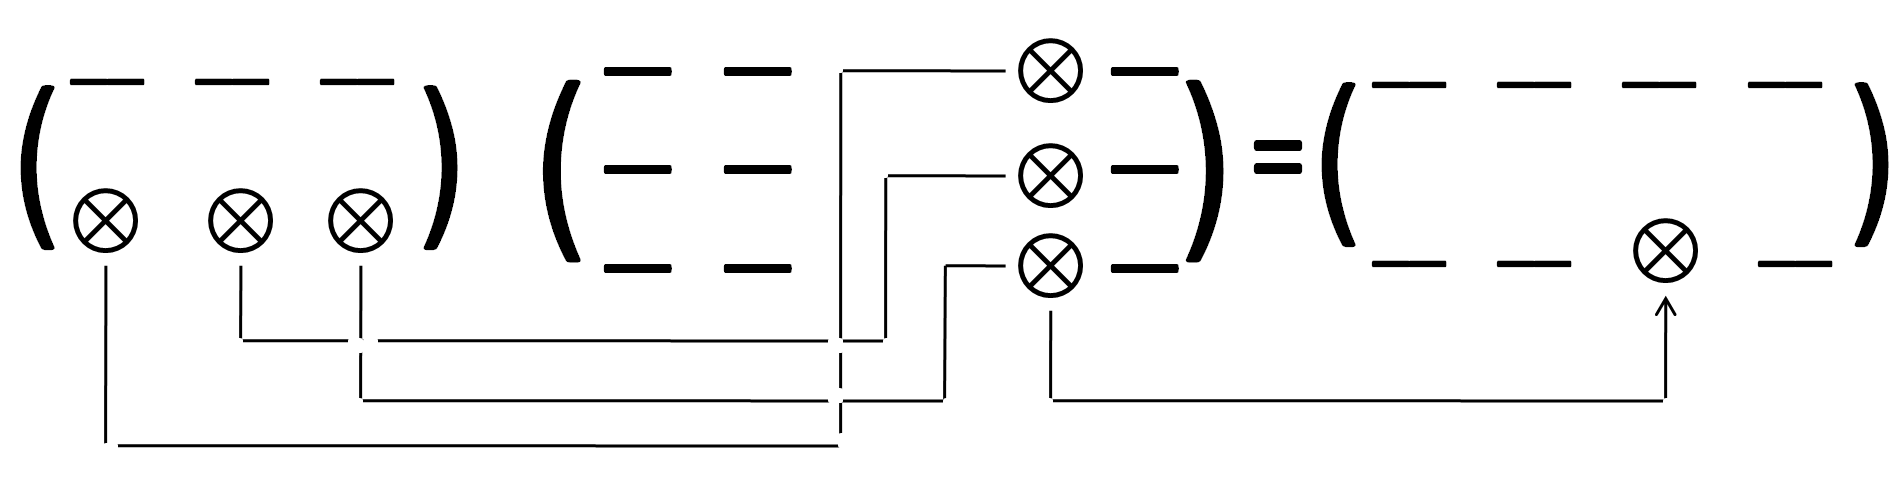
\includegraphics[scale=0.22]{./fig/3-0.png}
\end{figure}

\textbf{例1}

求下边矩阵的积。
\[
\begin{pmatrix}
    3 & 1 & 2 \\
    1 & 2 & 3
\end{pmatrix}
\begin{pmatrix}
    1 & 0 & 1 & 0 \\
    0 & 1 & 0 & 1 \\
    1 & 0 & 1 & 0
\end{pmatrix}    
=
\begin{pmatrix}
    C_{11} & C_{12} & C_{13} & C_{14} \\
    C_{21} & C_{22} & C_{23} & C_{24}
\end{pmatrix} 
\]
用方程3-15计算这八个矩阵元:
\[
\begin{array}{ll}
    C_{11}=3 \cdot 1+1 \cdot 0+2 \cdot 1=5 & C_{21}=1 \cdot 1+2 \cdot 0+3 \cdot 1=4 \\
    C_{11}=3 \cdot 0+1 \cdot 1+2 \cdot 0=1 & C_{21}=1 \cdot 0+2 \cdot 1+3 \cdot 0=2 \\
    C_{11}=3 \cdot 1+1 \cdot 0+2 \cdot 1=5 & C_{21}=1 \cdot 1+2 \cdot 0+3 \cdot 1=4 \\
    C_{11}=3 \cdot 0+1 \cdot 1+2 \cdot 0=1 & C_{21}=1 \cdot 0+2 \cdot 1+3 \cdot 0=2
\end{array}    
\]
其积为
\[
\begin{pmatrix}
    5 & 1 & 5 & 1  \\
    4 & 2 & 4 & 2
\end{pmatrix}    
\]
同学们应验证一下这些矩阵元,同时也可巩固乘二矩阵的“食指法”。

\vspace{0.5cm}

\textbf{例2}

求下列二方阵的积。
\[
\begin{pmatrix}
    1 & 2 \\
    3 & 4
\end{pmatrix}      
\begin{pmatrix}
    4 & 3 \\
    2 & 1
\end{pmatrix} 
=
\begin{pmatrix}
    8 & 5 \\
    20 & 13
\end{pmatrix}   
\]

矩阵相乘的另一特殊性质是不可对易性。标量相乘,标量和矩阵相加都是可对易的运算:$ab=ba,a+b=b+a,A+B=B+A$一般讲,矩阵相乘是不可对易的:$AB \neq BA$。
因为非方阵不能从个方向相乘,所以我们只考虑方阵的对易问题。在例2中,
\[
\begin{pmatrix}
    1 & 2 \\
    3 & 4
\end{pmatrix}      
\begin{pmatrix}
    4 & 3 \\
    2 & 1
\end{pmatrix} 
=
\begin{pmatrix}
    8 & 5 \\
    20 & 13
\end{pmatrix}   
\neq
\begin{pmatrix}
    13 & 20 \\
    5 & 8
\end{pmatrix}   
=   
\begin{pmatrix}
    4 & 3 \\
    2 & 1
\end{pmatrix} 
\begin{pmatrix}
    1 & 2 \\
    3 & 4
\end{pmatrix}   
\]

继续讨论矩阵的初等算术。下面介绍与数相似的两个矩阵。矩阵元全为零的矩阵叫做零矩阵,0。和数零相似,零知比加任何矩阵(同维)仍得该矩阵:
\[A+0=A \tag{3-17}\]

对角元全为一,非对角元全为零的矩阵(方阵)叫做恒等或单位矩阵,$E$(或记着$I$或$1$)。用克朗尼克符号可使此定义很简洁。我们义定
\[e_{ii}=1 \tag{3-18a}\]
对全部$i$,
\[e_{ij}=1 \tag{3-18a}\]
对全部$i \neq j$。这和定义
\[e_{ij}=\delta_{ij}\]
等价。只对方阵定义的恒等矩阵具有与数一相似的性质,即$E$与任何矩阵(方阵并与E同维)的积仍为该矩阵: $EA=A$。

做为使用一般化公式(方程3-15)的练习,我们证明$E$与所有矩阵都可对易。积$EA$的$ij$矩阵元是
\[(EA)_{ij}=\sum_ke_{ik}a_{kj}=\sum_k\delta_{ik}a_{kj}=a_{ij} \tag{3-19}\]
而
\[(AE)_{ij}=\sum_ka_{kj}e_{ik}=\sum_ka_{kj}\delta_{ik}=a_{ij}=(EA)_{ij} \tag{3-19}\]
既然有与数一的性质相似的矩阵,那么是否也有与倒数(因而与商)相似的矩阵?

\begin{definition}[逆矩阵]
    方阵$A$的逆矩阵(记着$A^{-1}$)是遵守下列关系的矩阵:
    \[A^{-1}A=AA^{-1}=E\]
    只对方阵定义逆矩阵。
\end{definition}

我们将讨论求逆矩阵的两个方法。第一个方法与上节介绍的检验线性无关的方法相似。第二个方法是用行列式定义的,我们稍后再讨论。行等价概念是找到第一个方法的线索。

\begin{theorem}[矩阵求逆]
    只有其行是线性无关的方阵$A$才有逆。可用下列步骤求逆。对$A$实施初等行运算使之变成$E$。然后以相同的顺序对$E$实施相同的行运算使之成$A^{-1}$。
\end{theorem}

应注意,一矩阵即便是非零矩阵也不定有逆。

正如上节的定理提示的那样,只有方阵$A$的行线性无关,$A$才是$E$的行等价矩阵。本定理的证明留给感兴趣的读者到许多好的代数教科书中去查找。我们只用一例来说明。

\textbf{例}

求下列方阵$A$的逆:
\[A=
\begin{pmatrix}
    1 & 2 \\
    3 & 4
\end{pmatrix} 
\]
先对$A$实施初等行运算使之成$E$:
\[
\begin{pmatrix}
    1 & 2 \\
    3 & 4
\end{pmatrix}    
\xrightarrow{r_2-3r_1}
\begin{pmatrix}
    1 & 2 \\
    0 & -2
\end{pmatrix} 
\xrightarrow{-\frac{1}{2} \cdot r_2}
\begin{pmatrix}
    1 & 2 \\
    0 & 1
\end{pmatrix} 
\xrightarrow{r_1-2r_2}
\begin{pmatrix}
    1 & 0 \\
    0 & 1
\end{pmatrix} 
=E
\]
然后对$E$实施相同运算:
\[
\begin{pmatrix}
    1 & 0 \\
    0 & 1
\end{pmatrix}
\xrightarrow{r_2-3r_1}
\begin{pmatrix}
    1 & 0 \\
    -3 & 1
\end{pmatrix}
\xrightarrow{-\frac{1}{2} \cdot r_2}
\begin{pmatrix}
    1 & 0 \\
    \frac{3}{2} & -\frac{1}{2}
\end{pmatrix}
\xrightarrow{r_1-2r_2}
\begin{pmatrix}
    -2 & 1 \\
    \frac{3}{2} & -\frac{1}{2}
\end{pmatrix}
=A^{-1}
\]
将答案乘以$A$以验证之:
\[
\begin{pmatrix}
    -2 & 1 \\
    \frac{3}{2} & -\frac{1}{2}
\end{pmatrix}   
\begin{pmatrix}
    1 & 2 \\
    3 & 4
\end{pmatrix} 
=
\begin{pmatrix}
    1 & 0 \\
    0 & 1
\end{pmatrix} 
\]
这种技巧既麻烦又易出错;同学们将会发现用行列式技巧比较保险。我们再用一个定义结束矩阵代数的讨论。

\begin{definition}[矩阵转置]
    方阵$A$的转置记为$A'$,其矩阵元
    \[a_{ij}'=a_{ji}\]
    以$A$的对角线为轴将矩阵翻转可得出$A'$。
\end{definition}

矩阵的转置在量子力学中很重要。转置的乘法遵守简单规则,
\[(AB)'=B'A' \tag{3-21}\]
若逆存在,它也遵守该规则,
\[(AB)^{-1}=B^{-1}A^{-1} \tag{3-22}\]

行列式。行列式的正式定义相当复杂,因此我们从使用行列式的实例开始。行列式的一个重要应用是解联立线性方程组。取下列方程组为例:
\[
\begin{array}{c}
    a_{11}x_1+a_{12}x_2=b_1 \\
    a_{21}x_1+a_{22}x_2=b_2
\end{array}    
\tag{3-23}
\]
将方程组写成这样形式就是要把我们引上以后要展开的矩阵观点。现在我们用代入法解方程3-23。
由第二个方程得$x_2=(b_2-a_{21}x_1)/a_{22}$,代入第一个方程,得出解
\[x_1=\frac{a_{22}b_1-a_{12}b_2}{a_{11}a_{22}-a_{12}a_{21}} \tag{3-24}\]
陈述式的分母包含联立方程组3-23的全部四个系数。事实上,分母就是称为系数矩阵的行列式。
\[A=
\begin{pmatrix}
    a_{11} & a_{12} \\
    a_{21} & a_{22} 
\end{pmatrix}
\tag{3-25a}
\]
\[
\begin{vmatrix}
    a_{11} & a_{12} \\
    a_{21} & a_{22} 
\end{vmatrix} 
\equiv
a_{11}a_{22}-a_{12}a_{21}
\tag{3-25b}
\]
方程3-24的分子也可写成行列式,因此结果为
\[
x_1=
\frac{
\begin{vmatrix}
    b_1 & a_{12} \\
    b_2 & a_{22} 
\end{vmatrix} 
}
{
\begin{vmatrix}
    a_{11} & a_{12} \\
    a_{21} & a_{22} 
\end{vmatrix} 
}   
\qquad 
x_2=
\frac{
\begin{vmatrix}
    a_{11} & b_1 \\
    a_{21} & b_2 
\end{vmatrix} 
}
{
\begin{vmatrix}
    a_{11} & a_{12} \\
    a_{21} & a_{22} 
\end{vmatrix} 
} 
\tag{3-26}
\]
此结果是以后要讨论的克拉姆规则的特例。方程3-25b给出$2 \times 2$行列式的简单定义。对应于大方阵的行列式的定义更复杂,不能从方程3-25b导出。
\begin{definition}[排列]
    $n$个整数的排列$P$是有序地排$n$个整数的一种方式;有$n!$个这样的排列。
    若排列中二指标换位数为偶;则P的符号为正;若排列中二指标换位数为奇,则$P$为负。
    \footnote{这里的二指标换位数定义应该与逆序数定义等价。}
\end{definition}
\textbf{例}

对整数$(1,2,3)$来讲,$(2,1,3)$是奇排列;$(2,3,1)$是偶排列。
\begin{definition}[行列式]
    方阵A的行列式记着$|A|$或$det \, A$;它是一个数(实数或复数),可用下式求出:
    \[|A|=\sum_{all \ P}^{n!}Sgn(P)a_{1,p_1}a_{2,p_2} \cdots a_{n,p_n} \tag{3-27}\]
\end{definition}
\textbf{例}

取$3 \times 3$行列式做为求行列式公式的例子。有$3!=6$项。求

\[
\begin{vmatrix}
    a_{11} & a_{12} & a_{13} \\
    a_{21} & a_{22} & a_{23} \\
    a_{31} & a_{32} & a_{33}
\end{vmatrix}    
\]
\[
\begin{tabular}{|c|c|c|c|}
    \hline
    项 & 排列 & 重排数 & Sgn(P) \\ \hline
    $a_{11} \ a_{22} \ a_{33}$ & 1 \ 2 \ 3 & 0 & + \\
    $a_{11} \ a_{23} \ a_{32}$ & 1 \ 3 \ 2 & 1 & - \\
    $a_{12} \ a_{21} \ a_{33}$ & 2 \ 1 \ 3 & 1 & - \\
    $a_{12} \ a_{23} \ a_{31}$ & 2 \ 3 \ 1 & 2 & + \\
    $a_{13} \ a_{22} \ a_{31}$ & 3 \ 2 \ 1 & 1 & - \\
    $a_{13} \ a_{21} \ a_{32}$ & 3 \ 1 \ 2 & 2 & + \\
    \hline
\end{tabular}
\]
以正确的符号\footnote{因个人技术能力有限,上表与原书有部分出入,基本想表达的思想应该是相同的。}将这些项加在一起,得出
\[|A|=a_{11}a_{22}a_{33}+a_{12}a_{23}a_{31}+a_{13}a_{21}a_{32}-a_{11}a_{23}a_{32}-a_{12}a_{21}a_{33}-a_{13}a_{22}a_{31} \tag{3-28}\]

这充其量也是一繁琐的步骤,但有比较简单的办法。将所有含$a_{11}$,$a_{12}$和$a_{13}$的项分别组合在一起,可得到简单办法的线索。
\[|A|=a_{11}(a_{22}a_{33}-a_{23}a_{32})+a_{12}(a_{23}a_{31}-a_{21}a_{33})+a_{13}(a_{21}a_{32}-a_{22}a_{31}) \tag{3-29a}\]
\[
=a_{11}
\begin{vmatrix}
    a_{22} & a_{23} \\
    a_{32} & a_{33}
\end{vmatrix}  
-a_{12}
\begin{vmatrix}
    a_{21} & a_{23} \\
    a_{31} & a_{33}
\end{vmatrix}  
+a_{13}
\begin{vmatrix}
    a_{21} & a_{22} \\
    a_{31} & a_{32}
\end{vmatrix}  
\]
方程3-29a表明行列式展成余因式;方程3-29b表明行列式展成余子式。

\begin{definition}[余因式,余子式]
    $n \times n$方阵的矩阵元$a_{ij}$的余因式$A_{ij}$是用$(n-1) \times (n-1)$行列式表示的数,余因式与行列式$|A|$的关系为
    \[|A|=\sum_ja_{ij}A_{ij} \tag{3-30}\]
    对任一i皆可。$n \times n$方阵的矩阵元$a_{ij}$的余子式$M_{ij}$是用$(n-1) \times (n-1)$行列式表示的数,此行列式是将$A$的$i$行和$j$列去掉而形成的。余子式和余因式最多差一符号:
    \[A_{ij}=M_{ij}(-1)^{i+j}\]
\end{definition}

\textbf{例}

取$4 \times 4$矩阵的$2,3$余子式和余因式为例,去掉第二行,去掉第三列。
\[
A=
\begin{pmatrix}
    a_{11} & a_{12} & a_{13} & a_{14} \\
    a_{21} & a_{22} & a_{23} & a_{24} \\
    a_{31} & a_{32} & a_{33} & a_{34} \\
    a_{41} & a_{42} & a_{43} & a_{44} 
\end{pmatrix}    
\]
\[
M_{23}=
\begin{vmatrix}
    a_{11} & a_{12} & a_{14} \\
    a_{31} & a_{32} & a_{34} \\
    a_{41} & a_{42} & a_{44} 
\end{vmatrix}    
\]
\[
A_{23}=-
\begin{vmatrix}
    a_{11} & a_{12} & a_{14} \\
    a_{31} & a_{32} & a_{34} \\
    a_{41} & a_{42} & a_{44} 
\end{vmatrix}    
=(-1)^{2+3}M_{23}
\]

\begin{theorem}
    $n \times n$矩阵$A$的行列式可展成余因式或余子式:
    \[|A|=\sum_ja_{ij}A_{ij}=\sum_ja_{ij}(-1)^{i+j}M_{ij}\]
    对任何$i$皆可。
\end{theorem}

\textbf{例}

用展成余子式和直接用方程3-28求下列$3 \times 3$行列式的值。
\[
\begin{vmatrix}
    1 & 0 & 2 \\
    3 & 4 & -1 \\
    -2 & 1 & 1
\end{vmatrix}    
=1
\begin{vmatrix}
    4 & -1 \\
    1 & 1
\end{vmatrix} 
-0
\begin{vmatrix}
    3 & -1 \\
    -2 & 1
\end{vmatrix} 
+2
\begin{vmatrix}
    4 & -1 \\
    1 & 1
\end{vmatrix} 
=5-0+22=27
\]
\[=-3
\begin{vmatrix}
    0 & 2 \\
    1 & 1
\end{vmatrix} 
+4
\begin{vmatrix}
    1 & 2 \\
    -2 & 1
\end{vmatrix} 
-(-1)
\begin{vmatrix}
    1 & 0 \\
    -2 & 1
\end{vmatrix} 
=6+20+1=27
\]
\[
=-2
\begin{vmatrix}
    0 & 2 \\
    4 & -1
\end{vmatrix}     
-1
\begin{vmatrix}
    1 & 2 \\
    3 & -1
\end{vmatrix} 
+1
\begin{vmatrix}
    1 & 0 \\
    3 & 4
\end{vmatrix} 
=16+7+4=27
\]
\[(1)(4)(1)+(0)(-1)(-2)+(2)(3)(1)-(1)(-1)(1)-(0)(3)(1)-(2)(4)(-2)=4+0+6+1-0+16=27\]
例中第一个方程是展成第一行的余子式;第二个方程是展成第一行的余子式;第三个方程是展成第三行的余子式。最后一个方程是用方程3-28(方程3-27的特例)直接求算。

若行列式中有零,则如上例中第一个方程那样对余子式展开特别有利。

检验向量的线性无关的初等行运算,也可在求算行列式时用做辅助手段。

\begin{theorem}
    常数乘方阵的一行等于该常数乘矩阵的行列式。
\end{theorem}

将$A$展成行的余因式,
\[|A|=\sum_ja_{ij}A_{ij} \tag{3-31}\]
常数$c$乘第$i$行给出一新矩阵,其行列式为
\[|B|=\sum_jb_{ij}B_{ij}=\sum_jca_{ij}A_{ij}=c\sum_ja_{ij}A_{ij}=c|A| \tag{3-32}\]

\begin{theorem}
    矩阵的二行交换使该矩阵的行列式变号。
\end{theorem}

此结果能用行列式的般定义证明。不需详细论证就可看出,原矩阵的展开式和换行的矩阵的展开式中的所有的项皆相同。因指标有一附加交换,故项的符号都不同。从此定理可立刻得出一推论。

\begin{proposition}
    有二恒等行的方阵的行列式为零。
\end{proposition}

这是因为交换恒等行给出符号相反的行列式,而交换恒等行又必须给出相同的行列式。因此,$|A|=-|A|$,这只有在$|A|=0$时才成立。最后,可得出实施最末一个初等行运算的结果。

\begin{theorem}
    方阵的二行相加,其行列式不变。
\end{theorem}

这可用展开$B$的行列式来证明($A$的第$i$行加第$k$行形成$B$的第$i$行)。利用$B$的第$i$行的余因式。
\[|B|=\sum_jb_{ij}B_{ij}=\sum_j(a_{ij}+a_{kj})A_{ij}=\sum_ja_{ij}A_{ij}+\sum_ja_{kj}A_{ij} \tag{3-33}\]
第一项是将$|A|$展成$A$的第$i$行的余因式的展开式。第二项看起来象是展成余因式的展开式,但这只有矩阵$A$第$i$行和第4行恒等时才成立。因此,第二项表示具有二恒等行的行列式的余因式展开;该行列式为零。因此,$|B|=|A|$。

做为概括的方式,附表给出初等行运算对行列式的值的影响。
\[
\begin{tabular}{|c|c|}
    \hline
    初等行运算 & 对行列式值的影响 \\ \hline
    1、常数乘行 & 常数乘行列式 \\
    2、交换行 & 行列式变号 \\
    3、行相加 & 不变 \\
    \hline
\end{tabular}
\]

我们用另外两个重要结果结束对行列式的基本性质的讨论。

\begin{theorem}
    二方阵乘积的行列式是二方阵的行列式的乘积:$|AB|=|A| \cdot |B|$。

    方阵的行列式等于该矩阵的转置的行列式:$|A|=|A'|$
\end{theorem}

在分析行列式的一般定义的基础上可以证明后一定理。所的项相同,符号也都相同。此定理使我们能将行语言表示的结果同样地用列语言表示出来。下表给出这些表述,也做为对有行列式知识的归纳。
\footnote{对下列第一点行展开和列展开\[|A|=\sum_ja_{ij}A_{ij}=\sum_ja_{ij}(-1)^{i+j}M_{ij} \qquad |A|=\sum_ia_{ij}A_{ij}=\sum_ia_{ij}(-1)^{i+j}M_{ij}\]}
\[
\begin{tabular}{|c|c|}
    \hline
    行语言表述 & 类似的列语言表述 \\ \hline
    1、用行的余因式或余子式展开行列式 & 用列的余因式或余子式展开行列式 \\
    2、常数乘行就是常数乘行列式。 & 常数乘列就是常数乘行列式。 \\
    3、变换行,行列式变号。 & 变换列,行列式变号。 \\
    4、具有二恒等行的矩阵的行列式为零。 & 具有二恒等列的矩阵的行列式为零。 \\
    5、两行相加行列式不变。 & 两列相加行列式不变。 \\
    \hline
\end{tabular}
\]

在了解行列式性质的基础上,我们可用较简单的方法处理两个问题。检验向量(做为矩阵的行)的线性无关和逆矩阵这两个问题,都曾用行等价解决。这些方法都是烦杂的,特别对大矩阵是这样。直接应用行列式的性质则为解决这两个问题提供了简便的方法。

\begin{theorem}
    苦$|A| \neq 0$,则方阵$A$有逆;逆矩阵$A^{-1}$的$i,j$矩阵元为
    \[(A^{-1})_{ij}=\frac{A_{ij}'}{|A|}=\frac{A_{ji}}{|A|} \tag{3-34}\]
\end{theorem}

将$|A|$展成余因式:
\[a_{i1}A_{i1}+a_{i2}A_{i2}+ \cdots +a_{in}A_{in}=|A|=\sum_ja_{ij}A_{ij} \tag{3-35}\]
用处理方程3-33同样的原理令第二项为零,若$i \neq k$也可得出
\[\sum_ja_{kj}A_{kj}=0 \tag{3-36}\]
这些关系式可合并为
\[\sum_ja_{kj}\frac{A_{ij}}{|A|}=\delta_{ki} \tag{3-37}\]
式中$\delta_{ki}$是单位矩阵E的一个矩阵元。方程3-37左端像是\footnote{原文写成“象似”,似乎是原古写法。}矩阵乘积。若将余因式$A_{ij}$改写为转置矩阵的余因式$A_{ij}'$
\footnote{\[\left(\sum_ja_{kj}\frac{A_{ij}}{|A|}\right)'=\sum_ja_{kj}\frac{A_{ij}'}{|A|}=\delta_{ki}\]},则方程3-37左端就是矩阵乘积。又因
\[\sum_ja_{kj}a_{kj}^{-1}=\delta_{ki}\]
所以$A_{ij}'/|A|=a_{ij}^{-1}$。应注意,仅当$|A|$不为零时这些矩阵元才存在。这里的符号$a_{ij}^{-1}$不表示$1/a_{ij}^{-1}$,而表示矩阵$A^{-1}$的$i,j$矩阵元。这就为求逆矩阵提供了更直接的途径。仍用前例来说明。

\textbf{例}

求
$
\begin{pmatrix}
    1 & 2 \\
    3 & 4
\end{pmatrix}
$
的逆矩阵。

根据上边给出的公式,
\[a_{11}^{-1}=\frac{A_{11}'}{|A|}=\frac{4}{-2}=-2\]
\[a_{12}^{-1}=\frac{A_{12}'}{|A|}=\frac{-2}{-2}=1\]
\[a_{21}^{-1}=\frac{A_{21}'}{|A|}=\frac{-3}{-2}=\frac{3}{2}\]
\[a_{22}^{-1}=\frac{A_{22}'}{|A|}=\frac{1}{-2}=-\frac{1}{2}\]
因此,
\[
A^{-1}=
\begin{pmatrix}
    -2 & 1 \\
    \frac{3}{2} & -\frac{1}{2}
\end{pmatrix}    
\]
这和前边求出的结果一样。

最后,将由行等价导出的线性无关和逆矩阵的结果,与有关非零行列式和逆矩阵的结果结合起来,可以得出线性无关和非零行列式之间的关系。

\begin{theorem}
    当且仅当矩阵的行列式不为零,该方阵的行才是线性无关的。
\end{theorem}

联立线性方程组。可用矩阵和行列式代数法,有效地解联立线性方程组。我们将不加证明地叙述其结果,并用一些例子说明此方法。

在介绍该问题的过程中,可看到联立线性方程组能用一个矩阵方程表示。一组含$n$个未知数的$m$个方程既可写为
\[
\begin{array}{c}
    a_{11}x_1+a_{12}x_2+ \cdots +a_{1n}x_n=b_1 \\
    a_{21}x_1+a_{22}x_2+ \cdots +a_{2n}x_n=b_2 \\
    \vdots \\
    a_{m1}x_1+a_{m2}x_2+ \cdots +a_{mn}x_n=b_m \\
\end{array}    
\tag{3-38}
\]
也可用矩阵方程表示
\[AX=B \tag{3-39}\]
式中A是$m \times n$系数矩阵,$X$是$n \times 1$未知数矩阵,B是$m \times 1$常数矩阵:
\[
\begin{pmatrix}
    a_{11} & a_{12} & \cdots & a_{1n} \\
    a_{21} & a_{22} & \cdots & a_{2n} \\
    \vdots & \vdots & \ddots & \vdots \\
    a_{m1} & a_{m2} & \cdots & a_{mn} \\
\end{pmatrix}    
\begin{pmatrix}
    x_{1} \\
    x_{2} \\
    \vdots \\
    x_{n} \\
\end{pmatrix} 
=
\begin{pmatrix}
    b_{1} \\
    b_{2} \\
    \vdots \\
    b_{m} \\
\end{pmatrix} 
\tag{3-40}
\]
我们还要定义两个概念。

\begin{definition}[增广矩阵,齐次方程组]
    一组含$n$个未知数的$m$个联立方程的增广矩阵是一个$m \times (n+1)$矩阵,它是将$m \times 1$常数矩阵补加在$m \times n$系数矩阵的右边而形成的。
    例如,若$A$和$B$是方程3-40中的矩阵,则增广矩阵$*A$为
    \[
    *A=
    \begin{pmatrix}
        a_{11} & a_{12} & \cdots & a_{1n} & b_{1} \\
        a_{21} & a_{22} & \cdots & a_{2n} & b_{2} \\
        \vdots & \vdots & \ddots & \vdots & \vdots \\
        a_{m1} & a_{m2} & \cdots & a_{mn} & b_{m} \\
    \end{pmatrix}
    \tag{3-41}
    \]

    若矩阵$B$为零,则这组联立线性方程称为齐次联立线性方程组。
\end{definition}

几乎完全不加证明的一些结果,可用下列定理表示出。

\begin{theorem}
    一组含$n$个未知数的$n$个联立线性方程,若系数行列式不为零则有解。其解可由逆矩阵或克莱姆规则构成。
\end{theorem}

若$AX=B$,则$A^{-1}AX=A^{-1}B$。因此,若已知$A^{-1}$,则$X$的一整组解就可得出。但仅当$|A| \neq 0$时$A^{-1}$才存在。其结果为
\[X=A^{-1}B \tag{3-42}\]
其个别解为
\[x_i=\sum_j(A^{-1})_{ij}b_j=\sum_j\frac{A_{ji}}{|A|}b_j=\sum_j\frac{b_jA_{ji}}{|A|} \tag{3-43}\]
方程3-43中出现的和
\[\sum_ib_iA_{ji}\]
是第i列为常数矩阵B的行列式的列余因式展开。达实际上就是以大家熟悉的形式表示的克莱姆规则:
\[x_i=\frac{
\begin{vmatrix}
    a_{11} & \cdots & b_{1} & \cdots & a_{1n} \\
    a_{21} & \cdots & b_{2} & \cdots & a_{2n} \\
    \vdots & & \vdots & & \vdots \\
    a_{n1} & \cdots & b_{n} & \cdots & a_{nn} \\
\end{vmatrix}   
}{
|A|
}\tag{3-44}\]

\begin{theorem}
    一组含$n$个未知数的$m$个联立线性方程,$AX=B$,若$A$中线性无关的行数$r$与$^*A$中的线性无关的行数相等,则有解。$r$个未知数可用其余的$n-r$个未知数表示,这$n-r$个未知数可取任意值。

    一组含$n$个未知数的$m$个线性齐次方程,总有零解$X=0$。若系数矩阵$A$的线性无关行,比未知数少,则有不全为零的解。同样$r$个未知数可用其余的$n-r$个未知数表示,这$n-r$个未知数可取任意值。
\end{theorem}

我们用说明这些定理的例子结束本节。

\textbf{例1}

含二未知数的两个线性方程
\[\begin{array}{c}
    4x+4y=2 \\ 8x-2y=4
\end{array}\]
用克莱姆规则得出的解为
\[x=\frac{
\begin{vmatrix}
    2 & 4 \\
    4 & -2
\end{vmatrix}
}{
\begin{vmatrix}
    4 & 4 \\
    8 & -2
\end{vmatrix}
}
=\frac{-20}{-40}=\frac{1}{2}\]
\[y=\frac{
\begin{vmatrix}
    4 & 2 \\
    8 & 4
\end{vmatrix}
}{
\begin{vmatrix}
    4 & 4 \\
    8 & -2
\end{vmatrix}
}
=\frac{0}{-40}=0\]
根据$AX=C$,$x=A^{-1}C$,可得出矩阵解。系数矩阵的逆是
\[
\begin{pmatrix}
    \frac{1}{20} & \frac{1}{10} \\
    \frac{1}{5} & -\frac{1}{10} 
\end{pmatrix}    
\]
方程组的解为
\[
\begin{pmatrix}
    x \\ y 
\end{pmatrix} 
=
\begin{pmatrix}
    \frac{1}{20} & \frac{1}{10} \\
    \frac{1}{5} & -\frac{1}{10} 
\end{pmatrix}  
\begin{pmatrix}
    2 \\ 4 
\end{pmatrix} 
=
\begin{pmatrix}
    \frac{2}{20}+\frac{4}{10} \\
    \frac{2}{5}-\frac{4}{10} 
\end{pmatrix} 
=
\begin{pmatrix}
    \frac{1}{2} \\ 0 
\end{pmatrix} 
\]
此矩阵方程表示$x=\frac{1}{2}$, $y=0$。

\textbf{例2}

含二未知数的三个方程
\[
\begin{array}{c}
    4x+4y=2 \\ 8x-2y=4 \\ x+y=1
\end{array}
\]
系数矩阵
\[
\begin{pmatrix}
    4 & 4 \\
    8 & -2 \\
    1 & 1
\end{pmatrix}    
\]
的行等价矩阵为
\[
\begin{pmatrix}
    1 & 1 \\
    0 & 10 \\
    0 & 0
\end{pmatrix}    
\]
因而有二线性无关的行。增广矩阵
\[
\begin{pmatrix}
    4 & 4 & 2 \\
    8 & -2 & 4 \\
    1 & 1 & 1
\end{pmatrix}    
\]
的行等价矩阵为
\[
\begin{pmatrix}
    1 & 1 & \frac{1}{2} \\
    0 & 1 & 0 \\
    0 & 0 & 1
\end{pmatrix}    
\]
它有三个线性无关的行。因此,这组方程无解。

\textbf{例3}

含二未知数的三个方程
\[
\begin{array}{c}
    4x+4y=2 \\ 8x-2y=4 \\ 3x+\frac{1}{2}y=\frac{3}{2}
\end{array}
\]
系数矩阵
\[
\begin{pmatrix}
    4 & 4 \\
    8 & -2 \\
    3 & \frac{1}{2}
\end{pmatrix}    
\]
的行等价矩阵是
\[
\begin{pmatrix}
    1 & 1 \\
    0 & 1 \\
    0 & 0
\end{pmatrix}    
\]
因而有二线性无关的行。增广矩阵
\[
\begin{pmatrix}
    4 & 4 & 2 \\
    8 & -2 & 4 \\
    3 & \frac{1}{2} & \frac{3}{2}
\end{pmatrix}    
\]
的行等价矩阵为
\[
\begin{pmatrix}
    1 & 1 & \frac{1}{2} \\
    0 & 1 & 0 \\
    0 & 0 & 0
\end{pmatrix}    
\]
它也有二线性无关的行,因此这组方程有解。其解可由增广矩阵的任一行等价矩阵得出。用最后一个矩阵做向导写出矩阵方程
\[
\begin{pmatrix}
    1 & 1 \\
    0 & 1
\end{pmatrix}   
\begin{pmatrix}
    x \\ y
\end{pmatrix}  
=
\begin{pmatrix}
    \frac{1}{2} \\ 0
\end{pmatrix} 
\]
用一般技巧(见例1),解此方程,求出$x=\frac{1}{2}$, $y=0$,与例1的解相同。也可以说,因本例的方程是线性相关的,同时两个方程与例1的相同。所以这组方程的解与例1的解相同。

\textbf{例4}

含三个未知数的两个方程
\[
\begin{array}{c}
    x+y+z=2 \\ x-y-z=1
\end{array}
\]
系数矩阵
\[
\begin{pmatrix}
    1 & 1 & 1 \\
    1 & -1 & -1
\end{pmatrix}    
\]
有两个线性无关的行,因其行等价矩阵为
\[
\begin{pmatrix}
    1 & 1 & 1 \\
    0 & -2 & -2
\end{pmatrix}    
\]
增广矩阵
\[
\begin{pmatrix}
    1 & 1 & 1 & 2\\
    1 & -1 & -1 & 1
\end{pmatrix}    
\]
的行等价矩阵为
\[
\begin{pmatrix}
    1 & 1 & 1 & 2\\
    0 & -2 & -2 & -1
\end{pmatrix}    
\]
它也有二线性无关的行;因此,这组方程有解。和上例一样,解这组方程可求助于增广矩阵的行等价矩阵,写出矩阵方程
\[
\begin{pmatrix}
    1 & 1 & 1 \\
    0 & -2 & -2
\end{pmatrix}    
\begin{pmatrix}
    x \\ y \\ z
\end{pmatrix}   
=
\begin{pmatrix}
    x+y+z \\ -2y-2z
\end{pmatrix}  
=
\begin{pmatrix}
    2 \\ -1
\end{pmatrix} 
\]
由此可得$x=2-y-z$,$y+z=\frac{1}{2}$。其解为$x=\frac{3}{2}$,$z=\frac{1}{2}-y$。
有无穷个解。即每一可能的y值就有一解。可用代入原方程组的方法验证一般解,每代入一次就给出一恒等式。
$x=\frac{3}{2}$,$y=0$,$z=\frac{1}{2}$是一组解;$x=\frac{3}{2}$,$y=1$,$z=-\frac{1}{2}$是另一组解,以此类推。

\textbf{例5}

含三个未知数的两个方程
\[
\begin{array}{c}
    x+y+z=2 \\ x+y+z=1
\end{array}
\]
用观察法可清楚地看出这组方程无解。考察系数矩阵也可以证实此结果。系数矩阵
\[
\begin{pmatrix}
    1 & 1 & 1 \\
    1 & 1 & 1
\end{pmatrix}    
\]
的行等价矩阵是
\[
\begin{pmatrix}
    1 & 1 & 1 \\
    0 & 0 & 0
\end{pmatrix}    
\]
因此有一个线性无关的行。另一方面, 增广矩阵
\[
\begin{pmatrix}
    1 & 1 & 1 & 2\\
    1 & 1 & 1 & 1
\end{pmatrix}    
\]
的行等价矩阵为
\[
\begin{pmatrix}
    1 & 1 & 1 & 2\\
    0 & 0 & 0 & -1
\end{pmatrix}    
\]
它有二线性无关的行。因系数矩阵和增广矩阵的线性无关的行数不同,故这组方程无解。

\textbf{例6}

含三个未知数的三个齐次方程
\[
\begin{array}{c}
    3x+4y+z=0 \\ 2x+6y+4z=0 \\ x-y+z=0
\end{array}
\]
系数矩阵
\[
\begin{pmatrix}
    3 & 4 & 1 \\
    2 & 6 & 4 \\
    1 & -1 & 1
\end{pmatrix}    
\]
有一等于$30$的行列式,和三个线性无关的行,因此这组齐次方程只有零解$x=y=z=0$。

\textbf{例7}

含三个未知数的三个齐次方程
\[
\begin{array}{c}
    x+y+z=0 \\ x-y-z=0 \\ x+3y+3z=0
\end{array}
\]
系数矩阵的行列式
\[
\begin{vmatrix}
    1 & 1 & 1 \\
    1 & -1 & -1 \\
    1 & 3 & 3
\end{vmatrix}   
=0 
\]
因此,这组方程有解。为了求解,还要求助增广矩阵的行等价矩阵。增广矩阵
\[
\begin{pmatrix}
    1 & 1 & 1 & 0 \\
    1 & -1 & -1 & 0 \\
    1 & 3 & 3 & 0 
\end{pmatrix}   
\]
的行等价矩阵是
\[
\begin{pmatrix}
    1 & 1 & 1 & 0 \\
    0 & 1 & 1 & 0 \\
    0 & 0 & 0 & 0 
\end{pmatrix}   
\]
因而只有两个线性无关的行。由增广矩阵写出的矩阵方程的解是$x+y+z=0$, $y+z=0$。即一般解为$x=0$,$y=-z$。和以前一样有无穷个特解。一个解是零解$x=y=z=0$;另一可能解是$x=0$, $y=1$, $z=-1$。

\section{线性变换}
在第二章定义函数时,我们强调在某特定区间给定一独立变量值就有一函数值。变换就是这个概念的推广。

\begin{definition}[线性空间上的变换]
    设存在$n$个独立变量$x_i \ (i=1,2,\cdots,n)$,每个变量都分别定义在特定区间内,诸如$a_1≤x_1≤b_1$, $a_2≤x_2≤b_2$, $\cdots$。
    若存在$m$个因变量$y_i$,每个因变量都是独立变量$x_i$的单值函数,我们说存在着一个将$n$-维空间($n$空间\footnote{原文这里是“$n$-空间”,为保持形式上的统一故改成“$n$空间”})中的一域变到$m$-维空间(或$m$空间)中的变换。
    写出$y_i=T(x_i)$,它表示一组$y_i$值在$T$变换下是一组$x_i$值的像。我们用大写字母表示变换。
\end{definition}

为了继续讨论本章第一节建立的代数课题,我们只限于讨论线性变换。

\begin{definition}[空间上的变换]
    变换$A$是线性的,当
    \[1. \ A(x_i+x_j)=A(x_i)+A(x_j)\]
    \[2. \ A(cx_i)=cA(x_i)\]
    式中c是标量。
\end{definition}

这个定义包含着线性的两个方面,这在记忆中应该是很熟悉的。这两个方面暗示出线性变换的形式必须是
\[
\begin{array}{c}
    a_{11}x_1+a_{12}x_2+ \cdots +a_{1n}x_n=y_1 \\
    \vdots \qquad \qquad \vdots \qquad \qquad \quad \vdots \quad \qquad \vdots \\
    a_{m1}x_1+a_{m2}x_2+ \cdots +a_{mn}x_n=y_m
\end{array}    
\tag{3-45}
\]
用矩阵语言可写
\[AX=Y \tag{3-46}\]
式中$A$是$m \times n$矩阵,$X$是$n \times 1$矩阵,$Y$是$m \times 1$矩阵。
由于可用矩阵表示线性变换,因此前边讨论的矩阵代数可用来帮助我们理解线性变换的性质。引入秩这个词将使讨论简化。

\begin{definition}[秩]
    矩阵的秩是矩阵中线性无关行的最大数;换句话说,矩阵的秩是由矩阵元形成的最大非零行列式的维数。线性变换的秩等于表示线性变换的矩阵的秩。
\end{definition}

根据非零行列式和线性无关之间的关系,可建立秩的另一定义。先讲一般结论,然后用特例说明。

\begin{theorem}
    设$n$空间到$m$空间的一线性变换的秩为$r$,在$m$空间的像为用$m$空间的$m$个坐标表示的线性方程组描述的$r$维子空间。当变换的秩$r=m$时,则变换可将$n$空间映入整个$m$空间。
\end{theorem}

做为证明,考虑一表示线性变换的$m \times n$知阵。若矩阵中只有$r$行是线性无关的,则$m-r$行是线性相关的,这就意味着$m$空间里有$m-r$个坐标是线性相关的。
因此,$n$空间在$m$空间的像是在$r$-维子空间上,$r$-维子空间是用$m$个坐标表示的线性方机,

\textbf{例}

有一变换
\[
\left .
\begin{array}{c}
    x+y+z=u \\ x+y+z=v
\end{array}
\right \} 
T
\]
T的秩就是矩阵
\[
\begin{pmatrix}
    1 & 1 & 1 \\ 1 & 1 & 1 
\end{pmatrix}  
\]
的秩,该矩阵有一线性无关的行;因此,秩为一。事实上,因矩阵的行相同,故$u=v$。因此$xyz$空间在$uv$空间的像就是$u=v$线,这是$uv$空间里的一个一维子空间。

在同学们将要学习的量子力学中,很重视函数或向量的正交性和归一性, 因此我们特别注意能保持这些性质的变换。
在欧氏向量空间这类变换称为正交变换;在厄米向量空间这类变换称为酉变换。

\begin{definition}[正交变换和酉变换]
    正交变换保存欧氏向量空间中向量的长度(归一性)和正交性;酉变换保存厄米向量空间中向量的正交性和归一性。
\end{definition}

这个定义是基本的,但如不从变换的结构上解释也效用不大。变换的结构是变换矩阵的矩阵元之间的关系。对结构的考查又要用这个定义。
设有一完备的正交向量组$\{\phi^i\}$。我们知道,如方程3-11描述并讨论过那样,任意向量$\alpha$可用向量组$\{\phi^i\}$按下式展开:
\[\alpha=\sum_ia_i\phi^i \tag{3-47}\]
设用$\{\phi^i\}$展开$\alpha$并保存其长度和正交性。即设$\alpha$是第二个完备正交归一组$\{\psi^j\}$的成员$\alpha=\psi^j$。因此,
\[\psi^j=\sum_ia_{ji}\phi^i \tag{3-48}\]
在方程3-47中系数$a_{ji}$加上第二个指标$j$以示出它是向量组$\{\psi^j\}$中的哪个向量。逆展开也是可能的(在一个习题里有此说明),因此
\[\phi^i=\sum_kb_{ik}\psi^k \tag{3-49}\]
合并这两个方程,得出
\[\psi^j=\sum_ia_{ji}\phi^i=\sum_ia_{ji}\sum_kb_{ik}\psi^k=\sum_k \left ( \sum_ia_{ji}b_{ik} \right )\psi^k \tag{3-50}\]
因$\{\phi^i\}$是线性无关的,所以当
\[j=k, \ \sum_ia_{ji}b_{ik}=1 \quad \text{and} \quad j \neq k, \ \sum_ia_{ji}b_{ik}=0\]
时上式才成立。得出,
\[\sum_ia_{ji}b_{ik}=\delta_{jk} \tag{3-51}\]
若不用展开系数语言而用矩阵语言表述,则可得
\[AB=E \tag{3-52}\]
或
\[A=B^{-1} \tag{3-53}\]
这是不奇怪的。因由基组$\{\phi^i\}$到基组$\{\psi^i\}$的变换必须用其行列式不为零的方阵表示;因而应存在逆。因此,将逆变换与向量的逆展开联系起来是唯一合理的。

我们还未涉及在变换中保存向量的正交归一性的问题。方程3-53是在要求保存完备性的条件下得出的。
对于$\psi^i$的正交归一性在欧氏向量空间有下列关系:
\[\bra*{\psi^i}\ket*{\psi^j}=\delta_{ij}=\sum_k\sum_l\bra*{\phi^kb_{ik}}\ket*{\phi^lb_{jl}}=\sum_{kl}\bra*{\phi^k}\ket*{\phi^l}b_{ik}b_{jl}=\sum_{kl}\delta_{kl}b_{ik}b_{jl}=\sum_kb_{ik}b_{jk} \tag{3-54}\]
方程3-54几近矩阵乘积,但又不十分像。若再一次求助于转置的定义,就可导出,
\[\delta_{ij}=\sum_kb_{ik}b_{kj}' \tag{3-55}\]
它表示
\[BB'=E \tag{3-56}\]
或
\[B^{-1}=B' \tag{3-56}\]
我们已经证明了下列结果。

\begin{theorem}
    (a)正交矩阵的还是该正交矩阵的转置。\\
    (b)西矩阵的这是该矩阵的复共轭的转置。\\
    (c)正交矩阵或酉矩阵的行是正交归一向量组。\\
    (d)正交矩阵或酉矩阵的列是正交归一向量组。
\end{theorem}

对厄来向量只要在适当地方加上复共轭,仍可用推导方程3-54到3-57的方法证明(b)。由方程3-54能清楚地看出(c),(d)也类似。
正交变换或酉变换的结构的最后一个方面,是关于矩阵表示的行列式的一个表述。
我们知道对于正交变换$BB'=E$;因此,
\[|B||B'|=|E|=1 \tag{3-58}\]
因$|B'|=|B|$,故
\[|B|= \pm 1 \tag{3-59}\]
我们证明了下列定理和酉变换的类似的结果。

\begin{theorem}
    正交矩阵的行列式为$+1$或$-1$;
    
    酉矩阵的行列式的模为$1$。
\end{theorem}

正交变换的一个特殊的和有用的几何应用是二维和三维转动。先考虑二维转动。
若转动$\alpha$角,则$P$点移至$P'$点。$P'$的坐标为
\[
\begin{array}{c}
    x'=x\cos \alpha-y\sin\alpha \\ y'=x\sin\alpha+y\cos \alpha
\end{array}    
\tag{3-60}
\]
它是一组线性方程。转动变换可用矩阵语言表示为
\[
R_{point}=
\begin{pmatrix}
    \cos \alpha & -\sin\alpha \\
    \sin\alpha & \cos \alpha
\end{pmatrix}    
\tag{3-61}
\]
\begin{figure}[htbp]
    \centering
    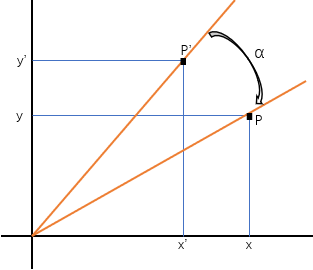
\includegraphics[scale=0.8]{./fig/3-1.png}
    \caption{在二位空间的转动}
\end{figure}
同学们应注意,在此过程中图3-1的坐标轴不动,而点动。此问题也可描述为坐标轴沿相反方向转动,即转$-\alpha$角:
\[
R_{axis}=
\begin{pmatrix}
    \cos \alpha & \sin\alpha \\
    -\sin\alpha & \cos \alpha
\end{pmatrix}    
\tag{3-62}
\]
存在着这两种观点,而应记住的一重要点是点的转动变换与坐标系转动的作用相反。

将二维转动变换的矩阵表示记住,现在观察三维转动。有许多考虑三维转动的方式,但所有这些方式都具有两个共同的原则。
第一,一般讲,需要用三个角来描述转动。读者对不对称物体做一演习就会相信这一点了。
第二,描述转动的习惯方式是按下列顺序:

(a)绕一坐标轴转$\phi$角。

(b)绕新位置的另一坐标轴转$\theta$角。

(c)再绕新位置的原坐标轴转$\psi$角。

这种转动顺序称为欧拉角转动(以数学家欧拉命名的)现代的作者们选择各种不同的顺序,因而同学们应小心地注意每一作者的习惯。为了和许多著名的教科书一致,我们的选择如图3-2所示。
\begin{figure}[htbp]
    \centering
    \begin{minipage}[t]{0.3\textwidth}
    \centering
    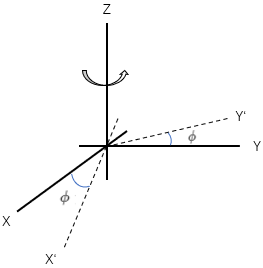
\includegraphics[width=4.5cm]{./fig/3-2a.png}
    (a)
    \end{minipage}
    \begin{minipage}[t]{0.3\textwidth}
    \centering
    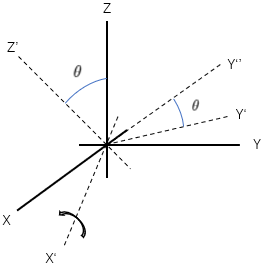
\includegraphics[width=4.5cm]{./fig/3-2b.png}
    (b)
    \end{minipage}
    \begin{minipage}[t]{0.3\textwidth}
    \centering
    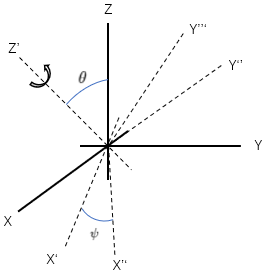
\includegraphics[width=4.5cm]{./fig/3-2c.png}
    (c)
    \end{minipage}
    \caption{在三维中转欧拉角(a)绕Z轴旋转$\phi(A)$; (b)绕X'轴旋转$\theta(B)$; (c)绕Z'轴旋转$\psi(C)$}
\end{figure}

(a)绕Z轴转$\phi$角得新的X'Y'Z坐标系(矩阵表示A)。

(b)绕X'轴转$\theta$角得新的X'Y''Z'坐标系\footnote{图B原书上Z'少了'。}(矩阵表示B)。

(c)绕Z'轴转$\psi$角得新的最终的X''Y'''Z'坐标系(矩阵表示C)。

此动作顺序表示坐标系转动。每一分步变换的矩阵表示可用与方程3-62类比的方法求出,它们是
\[A=
\begin{pmatrix}
    \cos \phi & \sin\phi & 0 \\
    -\sin\phi & \cos \phi & 0 \\
    0 & 0 & 1
\end{pmatrix}
\tag{3-63a}
\]
\[B=
\begin{pmatrix}
    1 & 0 & 0 \\
    0 & \cos \theta & \sin\theta \\
    0 & -\sin\theta & \cos \theta
\end{pmatrix}
\tag{3-63b}
\]
\[C=
\begin{pmatrix}
    \cos \psi & \sin\psi & 0 \\
    -\sin\psi & \cos \psi & 0 \\
    0 & 0 & 1
\end{pmatrix}
\tag{3-63c}
\]
三个分步转动的总效应给出一般化的三维转动矩阵$R=ABC$\footnote{因下式长度问题,这里稍微对原式做些许改动。},
\[R=
\begin{pmatrix}
    \cos \psi \cos \phi-\cos \theta \sin\phi \sin\psi & \cos \psi \sin\phi+\cos \theta \cos \phi \sin\psi & \sin\psi \sin\theta \\
    -\sin\psi \cos \phi-\cos \theta \sin\phi \cos \psi & -\sin\psi \sin\phi+\cos \theta \cos \phi \cos \psi & \cos \psi \sin\theta \\
    \sin\theta \sin\phi & -\sin\theta \cos \phi & \cos \theta
\end{pmatrix}
\tag{3-64}
\]
它虽然很复杂,但在讨论分子转动中很重要。

做为本节的总结和前两节的部分提纲,下表列出有关变换、矩阵、行列式和线性无关的表述之间的相互关系。同学们应努力掌握此课题的内在联系并应用它。
\begin{center}
    \textbf{等价表述; $n \times n$矩阵}\\
    \textbf{情况1. 行列式不为零}
\end{center}

1.向量组线性无关。

2.单位矩阵的行等价。

3.矩阵有逆。

4.矩阵的秩$r$等于维数$n$。

5.线性变换是$n$空间到$n$空间一对一的映射。

6.矩阵的行列式不为零。

7.含$n$个未知数的$n$个联立方程有解。

\begin{center}
    \textbf{情况2.行列式为零}
\end{center}

1.向量组线性相关。

2.是至少有一全为零的行的三角矩阵的行等价矩阵。

3.矩阵无逆。

4.矩阵的秩$r$小于维数$n$。

5.线性变换是$n$空间到$n$空间的$r$-维子空间的多对一的映射。

6.矩阵的行列式为零。

7.含$n$个未知数的$n$个齐次联立线性方程有解。

\begin{center}
    \textbf{等价表述:秩为$r$的$m \times n$矩阵}
\end{center}

1. $m$个向量中任何$r$个向量线性无关,$m-r$个向量是$r$个独立向量的因向量。

2.是有$m-r$个全为零的行的三角矩阵的行等价矩阵。

3.线性变换是$n$空间到$m$空间的$r$-维子空间的映射。

4.若增广矩阵的秩也是$r$,则联立线性方程组有解。

\section{线性算符}

本节在应用向量空间代数于量子力学方面将迈进主要的一步。早在第一章我们就讲过量子力学的本征值方程的作用,并见过这样方程所取的形式,如方程1-2。
虽然对特殊算符的描述要留给量子力学著作来讨论,但在这里能列出其一般结果。按我们的习惯先介绍一些定义。

\begin{definition}[算符]
    算符是定义在某向量空间变该空间中一向量为另一向量的一组指令。
    由此,我们写下$\mathscr{A}\xi=\eta$来表示,将体现在算符$\mathscr{A}$的定义中的一组特定指令作用于向量$\xi$形成一新向量$\eta$。用草体字表示算符。
\end{definition}

我们要问算符的这个定义和变换的定义之间有何区别。经最终分析可以说它们没有区别。
算符一词在量子力学的行文中常用于表示特定物理量,而变换一词则用于表示坐标系的改变。
无论如何,它们的定义在形式上是相同的,而且线性算符的定义和线性变换的定义也是相似的。

\begin{definition}[线性算符]
    线性算符服从下列方程:\\
    (a) $\mathscr{A}(c\xi)=c\mathscr{A}\xi$,式中$c$是常数(也可能是复数)。\\
    (b) $\mathscr{A}(\xi+\eta)=\mathscr{A}\xi+\mathscr{A}\eta$,式中$\xi$和$\eta$都是向量。
\end{definition}

算符表示“一组指令”这一定义并未给出表示算符的方式。那么怎样表示线性算符呢?
算符$\mathscr{A}$作用于任一向量的结果可从算符$\mathscr{A}$作用于基向量的结果求出。
例如,设已知
\[\mathscr{A}\phi^i=\sum_jA_{ij}\phi^j \tag{3-65}\]
式中向量组$\{\phi^i\}$,$\{\phi^j\}$是所讨论的向量空间中两组完备正交归一基向量组。
任一向量都可在$\{\phi^i\}$,$\{\phi^j\}$下展开\footnote{原文为“任一向量都可展开成$\phi^j$”,感觉翻译有问题。}:
\[\xi=\sum_ic_i\phi^i \qquad \eta=\sum_id_j\phi^j \tag{3-66}\]
我们再用算符定义$\mathscr{A}\xi=\eta$,将数$\{c_i\}$和$\{d_i\}$联系起来:
\[\mathscr{A}\xi=\mathscr{A}\sum_ic_i\phi^i=\sum_{ij}c_iA_{ij}\phi^j=\eta=\sum_jd_j\phi^j \tag{3-67}\]
因此,
\[d_j=\sum_iA_{ij}c_i \tag{3-68}\]
现在只需揭示出数$\{A_{ij}\}$是什么。若基向量$\{\phi^i\}$是正交归一的,那就容易办到,
\[\bra*{\phi^j}\ket*{\mathscr{A}\phi^i}=\sum_k\bra*{\phi^j}\ket*{A_{ik}\phi^k}=\sum_kA_{ik}\bra*{\phi^j}\ket*{\phi^k}=A_{ij} \tag{3-69}\]
我们时常见到方程3-69左边的那条竖线$\bra*{\phi^j}\mathscr{A}\ket*{\phi^i}$,此特殊竖线并未增加新的含义,只是提醒注意中心的算符$\mathscr{A}$。
像$\bra*{\phi^j}\mathscr{A}\ket*{\phi^i}$这样的内积常称为矩阵元。接下去我们就会看到使用这些矩阵元带来很大的方便。
例如,方程3-68现在可写成
\[d_j=\sum_i\bra*{\phi^j}\mathscr{A}\ket*{\phi^i}c_i \tag{3-70}\]
它具有矩阵乘积的形式\footnote{原书这里写得很乱,这里稍微修整了一下。},
\[
\begin{pmatrix}
    d_1 \\ d_2 \\ \vdots \\ d_n
\end{pmatrix}    
=
\begin{pmatrix}
    \bra*{\phi^1}\mathscr{A}\ket*{\phi^1} & \bra*{\phi^1}\mathscr{A}\ket*{\phi^2} & \cdots & \bra*{\phi^1}\mathscr{A}\ket*{\phi^n} \\
    \bra*{\phi^2}\mathscr{A}\ket*{\phi^1} & \bra*{\phi^2}\mathscr{A}\ket*{\phi^2} & \cdots & \bra*{\phi^2}\mathscr{A}\ket*{\phi^n} \\
    \vdots & \vdots & \ddots & \vdots \\
    \bra*{\phi^n}\mathscr{A}\ket*{\phi^1} & \bra*{\phi^n}\mathscr{A}\ket*{\phi^2} & \cdots & \bra*{\phi^n}\mathscr{A}\ket*{\phi^n}
\end{pmatrix}
\begin{pmatrix}
    c_1 \\ c_2 \\ \vdots \\ c_n
\end{pmatrix} 
\tag{3-71}
\]
在此情况下我们除去了展开系数$A_{ij}$(小体大写字母),并代之以通常的矩阵元$a_{ji}=\bra*{\phi^j}\mathscr{A}\ket*{\phi^i}$:
\[d_j=\sum_iA_{ij}c_i=\sum_ia_{ji}c_i \tag{3-72}\]
在这里我们用列矩阵($n \times 1$矩阵)表示向量。若左向量写成$1 \times n$行矩阵在向量写成$n \times 1$列矩阵,则内积可由用矩阵符号表示的二向量形成。它们的乘积自然是$1 \times 1$矩阵或标量:
\[\bra*{\xi}\ket*{\eta}=\left(c_1^* \ c_2^* \ \cdots \ c_n^*\right)
\begin{pmatrix}
    d_1 \\ d_2 \\ \vdots \\ d_n
\end{pmatrix}
=\sum_{i=1}^nc_i^*d_i \tag{3-73}\]
在我们讨论的情况,$\eta=\mathscr{A}\xi$。因此,
\[\bra*{\xi}\ket*{\eta}=\bra*{\xi}\mathscr{A}\ket*{\xi}=\left(c_1^* \ c_2^* \ \cdots \ c_n^*\right)
\begin{pmatrix}
    a_{11} & a_{12} & \cdots & a_{1n} \\
    a_{21} & a_{22} & \cdots & a_{2n} \\
    \vdots & \vdots & \ddots & \vdots \\
    a_{n1} & a_{n2} & \cdots & a_{nn}
\end{pmatrix}
\begin{pmatrix}
    d_1 \\ d_2 \\ \vdots \\ d_n
\end{pmatrix}
\tag{3-74}\]

现在出现了两个重要特点。用方阵表示线性算符和用列矩阵表示向量。
由于定义矩阵元为$a_{ji}=\bra*{\phi^j}\mathscr{A}\ket*{\phi^i}$,故所用的矩阵依赖于基组$\{\phi^i\}$的选择。
当然任何基组都可用。因此,有许多表示$\mathscr{A}$的矩阵,不同的矩阵表示产生于不同的基。
因此,严格讲,说算符$\mathscr{A}$与其矩阵元为$a_{ij}$的矩阵$A$相同是不正确的;
应该说,矩阵表示$\mathscr{A}$,或矩阵是算符$\mathscr{A}$的以$\{\phi^i\}$为基的表示。
同样地,说$\eta$与列向量
\[
\begin{pmatrix}
    d_1 \\ d_2 \\ \vdots \\ d_n
\end{pmatrix}
\]
相同也是不正确的,应该说,此列向量是$\eta$的表示或此列向量表示$\eta$。

我们还应考察一给定算符的二矩阵表示之间的关系。令$A^{\phi}$为$\mathscr{A}$的以$\{\phi^i\}$为基的表示,$A^{\psi}$为$\mathscr{A}$的以$\{\psi^i\}$为基的表示。
矩阵元为$a_{ij}^{\phi}=\bra*{\phi^i}\mathscr{A}\ket*{\phi^j}$和$a_{ij}^{\psi}=\bra*{\psi^i}\mathscr{A}\ket*{\psi^j}$。又设二基(正交归一的)以酉变换
\[\psi^i=\sum_ku_{ik}\phi^k\]
相关联,反过来,
\[\phi^i=\sum_ju^*_{ji}\psi^j=\sum_ju'^*_{ij}\psi^j\]
于是,矩阵元$a_{ij}^{\phi}$与$a_{ij}^{\psi}$之间的关系为
\[a_{ij}^{\psi}=\bra*{\psi^i}\mathscr{A}\ket*{\psi^j}=\sum_ku^*_{ik}\bra*{\phi^k}\mathscr{A}\ket*{\psi^j}=\sum_{kl}u^*_{ik}u_{jl}\bra*{\phi^k}\mathscr{A}\ket*{\phi^l}=\sum_{kl}u^*_{ik}u_{jl}a_{kl}^{\phi}\]
\[=\sum_{kl}u_{ik}'^{-1}a_{kl}^{\phi}u_{lj}'=[U'^{-1}A^{\phi}U']_{ij} \tag{3-75}\]
结构$A^{\psi}=U'^{-1}A^{\phi}U'$经常出现在代数方程组中。若$A=S^{-1}BS$,我们就说对B进行相似变换得到A。
若$S$是酉矩阵(现在$S=U'$),则变换称为酉变换。由此得出下列结果。

\begin{theorem}
    $\mathscr{A}$的以$\psi$为基的矩阵表示可通过对$\mathscr{A}$的以$\phi$为基的矩阵表示作相似变换得出;这个相似变换就是联系二基的变换的转置。
\end{theorem}

我们建立了线性算符和它们的矩阵表示之间的关系;它只是矩阵代数的概念,矩阵乘积,逆矩阵和转置矩阵对算符的自然推广。还有一些概念很重要,它们包含在下列定义中。

\begin{definition}[换位子,伴算子]
    二算符$\mathscr{A}$和$\mathscr{B}$的换位子是$\mathscr{A}\mathscr{B}-\mathscr{B}\mathscr{A}$,记着$[\mathscr{A},\mathscr{B}]$。
    算符$\mathscr{A}$的伴算符,记着$\mathscr{A}^{\dagger}$,其矩阵元和$\mathscr{A}$的矩阵元有如下关系:
    \[\bra*{\phi^i}\mathscr{A}^{\dagger}\ket*{\phi^j}=\bra*{\mathscr{A}\phi^i}\ket*{\phi^j}\]    
\end{definition}

$\mathscr{A}$的伴算符的矩阵是$\mathscr{A}$的矩阵表示转置并共轭化,因
\[\bra*{\phi^i}\ket*{\mathscr{A}^{\dagger}\phi^j}=\bra*{\mathscr{A}\phi^i}\ket*{\phi^j}=\bra*{\phi^j}\mathscr{A}\ket*{\phi^i}^* \tag{3-76}\]
剑号表示伴算符。

\begin{definition}[迹]
    算符的迹是算符的任何矩阵表示的对角元之和:
    \[\text{tr}\mathscr{A}=\sum_ia_{ii}\]
    (德语文献中迹称为Spur并简写为Sp)
\end{definition}

考虑一典型算符及其一些不同基的表示,做为已讨论的某些原则的例子。

\begin{definition}[投影算符]
    将某向量投影到一单位向量$\epsilon$的方向上的投影算符$\sigma_{\epsilon}$。定义为$\sigma_{\epsilon}\xi=\bra*{\epsilon}\ket*{\xi}\epsilon$。
\end{definition}

投影算符给出一向量在特定方向上的分量。应用算符法就能非常简便地解出$\sigma_{\epsilon}$的特征值:
\[\sigma_{\epsilon}^2\xi=\sigma_{\epsilon}(\sigma_{\epsilon}\xi)=\sigma_{\epsilon}(\bra*{\epsilon}\ket*{\xi}\epsilon)=\bra*{\epsilon}\ket*{\xi}\sigma_{\epsilon}\epsilon=\bra*{\epsilon}\ket*{\xi}\epsilon \tag{3-77}\]

因此,$\sigma_{\epsilon}^2=\sigma_{\epsilon}$。这表示算符$\sigma_{\epsilon}$是“幂等的”($idempotent$)由此可
得,$(\sigma_{\epsilon}^2-\sigma_{\epsilon})=0=\sigma_{\epsilon}(\sigma_{\epsilon}-1)=0$,即$\sigma_{\epsilon}=0$或$\sigma_{\epsilon}=1$。
即便不写出$\sigma_{\epsilon}$的矩阵表示,我们就已经知道$\sigma_{\epsilon}$的本征值(一或零)。
现在让我们看看$\sigma_{\epsilon}$的矩阵表示是什么样。

\textbf{例}

在二维欧氏向量空间投影方向向量为$\epsilon=(1/\sqrt{2},1/\sqrt{2})$的投影算符。
取习用的笛卡儿基$\phi^1=(1,0)$, $\phi^2=(0,1)$为基。用直接法得出
\[p_{11}^{\phi}=\bra*{\phi^1}\sigma\ket*{\phi^1}=\bra*{(1,0)}\ket*{\left(\frac{1}{\sqrt{2}},\frac{1}{\sqrt{2}}\right)\left(\frac{1}{\sqrt{2}}\right)}=\frac{1}{\sqrt{2}} \cdot \frac{1}{\sqrt{2}}=\frac{1}{2}\]
\[p_{12}^{\phi}=\frac{1}{2} \qquad p_{21}^{\phi}=\frac{1}{2} \qquad p_{22}^{\phi}=\frac{1}{2}\]
矩阵$P^{\phi}$为
\[
\begin{pmatrix}
    \frac{1}{2} & \frac{1}{2} \\ \frac{1}{2} & \frac{1}{2}
\end{pmatrix}    
\]
再考虑基$\psi^1=(1/2,\sqrt{3}/2)$, $\psi^2=(\sqrt{3}/2,-1/2)$的情况。用同样的计算方法,得出矩阵元$p_{ij}^{\psi}$和矩阵
\[P^{\psi}=
\begin{pmatrix}
    \frac{1}{2}+\frac{\sqrt{3}}{4} & \frac{1}{4} \\
    \frac{1}{4} & \frac{1}{2}-\frac{\sqrt{3}}{4}
\end{pmatrix}
\]
现在应验证一下变换定理,$P^{\psi}=U'^{-1}P^{\phi}U'$。因\footnote{原书下式第一个$\phi^2$的系数误写成了$\frac{\sqrt{2}}{2}$(笑)。}
\[\psi^1=\frac{1}{2}(1,0)+\frac{\sqrt{3}}{2}(0,1)=\frac{1}{2}\phi^1+\frac{\sqrt{3}}{2}\phi^2\]
\[\psi^2=\frac{\sqrt{3}}{2}(1,0)-\frac{1}{2}(0,1)=\frac{\sqrt{3}}{2}\phi^1-\frac{1}{2}\phi^2\]
所以
\[
U=
\begin{pmatrix}
    \frac{1}{2} & \frac{\sqrt{3}}{2} \\
    \frac{\sqrt{3}}{2} & -\frac{1}{2}
\end{pmatrix}
\qquad
U'=
\begin{pmatrix}
    \frac{1}{2} & \frac{\sqrt{3}}{2} \\
    \frac{\sqrt{3}}{2} & -\frac{1}{2}
\end{pmatrix}
U'^{-1}=
\begin{pmatrix}
    \frac{1}{2} & \frac{\sqrt{3}}{2} \\
    \frac{\sqrt{3}}{2} & -\frac{1}{2}
\end{pmatrix}
\]
直接相乘
\[
\begin{pmatrix}
    \frac{1}{2} & \frac{\sqrt{3}}{2} \\
    \frac{\sqrt{3}}{2} & -\frac{1}{2}
\end{pmatrix}   
\begin{pmatrix}
    \frac{1}{2} & \frac{1}{2} \\
    \frac{1}{2} & \frac{1}{2}
\end{pmatrix}
\begin{pmatrix}
    \frac{1}{2} & \frac{\sqrt{3}}{2} \\
    \frac{\sqrt{3}}{2} & -\frac{1}{2}
\end{pmatrix}
=
\begin{pmatrix}
    \frac{1}{2}+\frac{\sqrt{3}}{4} & \frac{1}{4} \\
    \frac{1}{4} & \frac{1}{2}-\frac{\sqrt{3}}{4}
\end{pmatrix}
=P^{\psi}
\]
我们可很快地求出,以$x^1=(1/\sqrt{2},1/\sqrt{2})$, $x^2=(1/\sqrt{2},1/\sqrt{2})$为基时$P$的形式为
\[
\begin{pmatrix}
    1 & 0 \\ 0 & 0
\end{pmatrix}    
\]
我们可以用这三个例子并结合图3-3(有点滑稽\footnote{确实(笑死)。})说明矩阵表示的概念。
\begin{figure}[htbp]
    \centering
    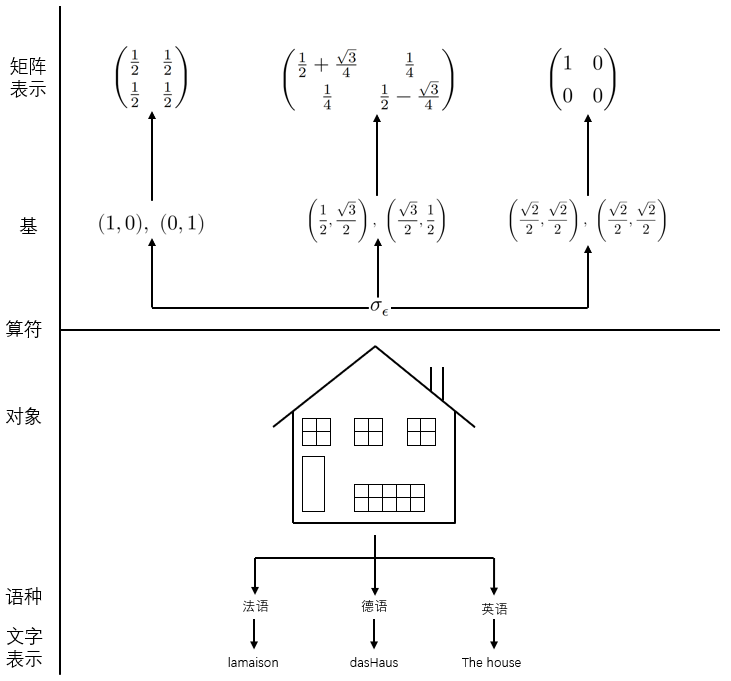
\includegraphics[scale=0.7]{./fig/3-3.png}
    \caption{算符$\sigma_{\epsilon}$, $\epsilon=(1/\sqrt{2},1/\sqrt{2})$及其在三个基上的矩阵表示;类比,对象房子,和在三个语种中的文字表示}
\end{figure}
最后我们讲,求线性算符的特征值和特征向量问题。井非所有线性算符都服从特征值方程,但从量子力学的观点看,有两类非常重要的算符服从特征值方程。
这些算符是厄米算符和酉算符,我们先概述一下结果,然后再证明。

\begin{definition}[简并特征值,简并度]
    若一特征值满足在同一个特征向量方程中对应多个特征向量\footnote{原文为“若一特征值满足多于一个特征向量的特征值一特征向量方程”,不知道翻译了个什么东西。},则称该特征值为简并的;特征值相同的特征向量数称为特征值的简并度。
\end{definition}

\begin{definition}[厄米算符]
    厄米算符是自伴的线性算符; 即$\mathscr{H}=\mathscr{H}^{\dagger}$或$h_{ij}=h_{ji}^*$。厄米矩阵的对角元是实的。
\end{definition}

\begin{theorem}
    在n维向量空间里的厄米算符有$n$个不同的特征向量和$n$个实特征值。
    若特征值是非简并的,则特征向量彼此正交,再乘以适合的归一化常数就形成正交归一向量组。
    即使某些特征向量是简并的,也可由不同的特征向量造正交归一组。
\end{theorem}

\begin{definition}[酉算符]
    酉算符是线性算符,其伴等于其逆:$\mathscr{U}^{-1}=\mathscr{U}^{\dagger}$。
\end{definition}

\begin{theorem}
    在n维向量空间的酉算符有$n$个不同的特征向量(如上,可形成正交归一组)和$n$个特征值,它们全都具有单位模。
\end{theorem}

我们从证明厄来定理开始。若$\mathscr{H}\phi^i=h_i\phi^i$,则$\bra*{\phi^i}\mathscr{H}\ket*{\phi^i}=h_i\bra*{\phi^i}\ket*{\phi^i}$。
因$\mathscr{H}$是厄米的,所以$\bra*{\phi^i}\mathscr{H}\ket*{\phi^i}=\bra*{\phi^i}\mathscr{H}\ket*{\phi^i}^*$, $h_i=h_i^*$,因而$h_i$是实的。
对于二不同的特征向量,
\[\mathscr{H}\phi^i=h_i\phi^i \tag{3-78a}\]
\[\mathscr{H}\phi^j=h_j\phi^j \tag{3-78a}\]
从方程3-78a得出$\bra*{\phi^i}\mathscr{H}\ket*{\phi^i}=h_i\bra*{\phi^i}\ket*{\phi^i}$;
从方程3-78b得出$\bra*{\mathscr{H}\phi^j}\ket*{\phi^i}=h_j^*\bra*{\phi^j}\ket*{\phi^i}$。
然而,$\bra*{\mathscr{H}\phi^j}\ket*{\phi^i}=\bra*{\phi^i}\mathscr{H}\ket*{\phi^j}^*=\bra*{\phi^j}\ket*{\mathscr{H}\phi^i}=h_i\bra*{\phi^j}\ket*{\phi^i}$
因此$(h_i-h_j^*)\bra*{\phi^j}\ket*{\phi^i}=0$,因$h_j$为实的,
当$h_i \neq h_j$时,则$\bra*{\phi^j}\ket*{\phi^i}=0$,因而特征向量是正交的。

对酉算符定理的证明很相似。若$\mathscr{U}\psi^i=u_i\psi^i$,则$\mathscr{U}^{\dagger}\mathscr{U}\psi^i=\mathscr{U}^{\dagger}u_i\psi^i=u_i\mathscr{U}^{\dagger}\psi^i$。
因此$\mathscr{U}^{\dagger}\psi^i=\left(\frac{1}{u_i}\right)\psi^i$或$\mathscr{U}^{\dagger}$的特征向量和$\mathscr{U}$的特征向量相同,而其特征值是$\mathscr{U}$的特征值的倒数。
于是,$\bra*{\psi^i}\mathscr{U}^{\dagger}\ket*{\psi^i}=u_i\bra*{\psi^i}\ket*{\psi^i}$, $\bra*{\mathscr{U}^{\dagger}\psi^i}\ket*{\psi^i}=(1/u_i^*)\bra*{\psi^i}\ket*{\psi^i}$。
但$\bra*{\mathscr{U}^{\dagger}\psi^i}\ket*{\psi^i}$又等于$\bra*{\psi^i}\mathscr{U}^{\dagger}\ket*{\psi^i}$,因此$1/u_i^*=u_i$, $u_i^*u_i=1$,或特征值$u_i$的模为一。
可用证明厄来算符类似的方法证明特征向量的正交性。由简并特征值产生的特殊问题在本节末讨论。

这些证明都未说明厄米算符或酉算符为什么必须服从特征值方程,现在只给结果而不加证明。无论如何,这些定理中的每一个都有在欧氏向量空间中的推论。
\begin{proposition}
    对应于厄米向量空间中的厄米算符定理,在欧氏向量空间中有一对称算符$(\delta_{ij}=\delta_{ji})$的类似定理;
    对应于厄米向量空间中的酉算符定理,在欧氏向量空间中有一正交算符$(\mathfrak{R}'=\mathfrak{R}^{-1})$的类似的定理。
\end{proposition}

所有定理和推论涉及的都是特征值和特征向量的存在问题,但到目前为止还未讲如何求这些本征值。
我们能够从两个观点(久期方程和相似变换)来研究解特征值方程的一般形式。

考虑一矩阵形式的特征值方程,方程1-2,
\[\mathfrak{Q}\phi=q\phi \tag{3-79}\]
此方程是许多用向量$\phi$的分量表示的线性方程的简要陈述:
\[
\begin{array}{c}
    \mathfrak{Q}_{11}\phi_1+\mathfrak{Q}_{12}\phi_2+ \cdots +\mathfrak{Q}_{1n}\phi_n=q\phi_1 \\
    \vdots \qquad \qquad \vdots \qquad \qquad \qquad \vdots \quad \qquad \vdots \\
    \mathfrak{Q}_{n1}\phi_1+\mathfrak{Q}_{n2}\phi_2+ \cdots +\mathfrak{Q}_{nn}\phi_n=q\phi_n \\
\end{array}    
\tag{3-80}
\]
将这些方程重新整理一下,可得一组含$n$个未知数$\phi_i$($\phi$的分量)的齐次联立方程:
\[
\begin{array}{c}
    (\mathfrak{Q}_{11}-q)\phi_1+\mathfrak{Q}_{12}\phi_2+ \cdots +\mathfrak{Q}_{1n}\phi_n=0 \\
    \mathfrak{Q}_{11}\phi_1+(\mathfrak{Q}_{12}-q)\phi_2+ \cdots +\mathfrak{Q}_{1n}\phi_n=0 \\
    \vdots \\
    \mathfrak{Q}_{n1}\phi_1+\mathfrak{Q}_{n2}\phi_2+ \cdots +(\mathfrak{Q}_{nn}-q)\phi_n=0 \\
\end{array}  
\tag{3-81}  
\]
我们已经学过,仅当系数行列式等于零时,这样的方程才有非全零解。由此得到的$q$的$n$次方程,称为久期方程:
\[
\begin{vmatrix}
    (\mathfrak{Q}_{11}-q) & \mathfrak{Q}_{12} & \cdots & \mathfrak{Q}_{1n} \\
    \mathfrak{Q}_{11} & (\mathfrak{Q}_{12}-q) & \cdots & \mathfrak{Q}_{1n} \\
    \vdots  & \vdots & \ddots  & \vdots \\
    \mathfrak{Q}_{n1} & \mathfrak{Q}_{n2} & \cdots & (\mathfrak{Q}_{nn}-q) \\
\end{vmatrix}    
=0 \tag{3-82}
\]
久期方程是量子力学中常见的方程。思考一下方程3-82的意义。若将方程3-82展开,可得到未知数$q$的$n$次多项式。
将解该方程的实际问题暂时放置一边,先注意出现的一个有意义的概念:方程有$n$个根。
前边证明了的定理说应有$n$个特征向量和$n$个特征值,现在看到了为什么。这是因为特征值是$n$次方程的解。
正如我们见过那样某些根当然可能相等,但我们不准备讨论此问题。

现在有$n$个特征值。对每个特征值可用方程组3-81解出特征向量的分量$\phi_i$。
因此,方程3-81最终给出$n$个特征向量,对每一特征值有一特征向量。
为了完成计算,还需将特征向量归一化。

概括讲,解矩阵特征值方程可用下列步骤:

1.写出并解久期方程;得出特征值。

2.将特征值(现在已知)代入特征值方程解出特征向量。

3.将特征向量归一化。

我们也可用第二个观点讨论特征值问题。假定我们已知矩阵的特征值和特征向量:
\[
\begin{array}{c}
    \mathfrak{Q}\phi^1=q_1\phi^1 \\
    \mathfrak{Q}\phi^2=q_2\phi^2 \\
    \vdots \quad \qquad \vdots \\
    \mathfrak{Q}\phi^n=q_n\phi^n 
\end{array}    
\tag{3-83}
\]
可将列向量一列挨一列排起来形成$n \times n$矩阵,如
\[
\Phi=
\begin{pmatrix}
    \phi^1_1 & \phi^2_1 & \cdots & \phi^n_1 \\
    \phi^1_2 & \phi^2_2 & \cdots & \phi^n_2 \\
    \vdots & \vdots & \ddots & \vdots \\
    \phi^1_n & \phi^2_n & \cdots & \phi^n_n 
\end{pmatrix}    
\tag{3-84}
\]
本征向量$\phi^i$形成矩阵$\Phi$的列。$\mathfrak{Q}$对$\Phi$作用产生其列为$q_i\phi^i$的矩阵:
\[
\mathfrak{Q}\Phi=
\begin{pmatrix}
    q_1\phi^1_1 & q_2\phi^2_1 & \cdots & q_n\phi^n_1 \\
    q_1\phi^1_2 & q_2\phi^2_2 & \cdots & q_n\phi^n_2 \\
    \vdots & \vdots & \ddots & \vdots \\
    q_1\phi^1_n & q_2\phi^2_n & \cdots & q_n\phi^n_n 
\end{pmatrix}  
=
\begin{pmatrix}
    \phi^1_1 & \phi^2_1 & \cdots & \phi^n_1 \\
    \phi^1_2 & \phi^2_2 & \cdots & \phi^n_2 \\
    \vdots & \vdots & \ddots & \vdots \\
    \phi^1_n & \phi^2_n & \cdots & \phi^n_n 
\end{pmatrix}
\begin{pmatrix}
    q_1 & 0 & \cdots & 0 \\
    0 & q_2 & \cdots & 0 \\
    \vdots & \vdots & \ddots & \vdots \\
    0 & 0 & \cdots & q_n
\end{pmatrix}
=\Phi \hat{q}
\tag{3-85}
\]
式中符号$\hat{q}$表示其对角元为$n$个特征值,其它矩阵元皆为零的矩阵。方程3-85两边皆乘以$\Phi^{-1}$给出,
\[\Phi^{-1}\mathfrak{Q}\Phi=\hat{q} \tag{3-86}\]
此式可表述如下:用由特征向量为列形成的矩阵对$\mathfrak{Q}$作相似变换,给出由$\mathfrak{Q}$的特征值形成的对角矩阵。

因此,若能找到将$\mathfrak{Q}$变换成对角矩阵方法(这叫做将矩阵$\mathfrak{Q}$对角化),则该相似变换的列是特征向量,对角矩阵的对角元是特征值。
这种步骤易为数学计算用,因而经常形成用计算机解特征值问题的基础。正如前边已证明那样,因向量$\phi^i$是正交归一的,故变换$\Phi^{-1}\mathfrak{Q}\Phi$是酉变换。
我们用求上边讨论过的$\sigma_{\epsilon}$。矩阵的特征值做为这些概念的例子。

\textbf{例}

考虑算符$\sigma_{\epsilon}$,其中$\epsilon=(1/\sqrt{2},1/\sqrt{2})$是取常用的笛卡儿基。投影算符在此基上的矩阵表示为前边求出那样是
\[
\begin{pmatrix}
    \frac{1}{2} & \frac{1}{2} \\ \frac{1}{2} & \frac{1}{2}
\end{pmatrix}    
\]
为了求此算符的特征值,我们解久期方程。
\[
\begin{vmatrix}
    \frac{1}{2}-p & \frac{1}{2} \\ \frac{1}{2} & \frac{1}{2}-p
\end{vmatrix}    
=0
\]
展开给出二次多项式。
\[\frac{1}{4}-p+p^2-\frac{1}{4}=0\]
它的根是
\[p^2-p=0\]
\[p_1=1, \ p_2=0\]
这些根是$\sigma_{\epsilon}$的特征值,这正是前边单独根据算符性质所预言的那样。我们现在求对应于特征值$p_1=1$的特征向量$\phi^1$:
\[
\begin{pmatrix}
    \frac{1}{2} & \frac{1}{2} \\ \frac{1}{2} & \frac{1}{2}
\end{pmatrix} 
\begin{pmatrix}
    \phi_1^1 \\ \phi_2^1
\end{pmatrix} 
= 
\begin{pmatrix}
    \phi_1^1 \\ \phi_2^1
\end{pmatrix}  
\]
可写为
\[\frac{1}{2}\phi_1^1+\frac{1}{2}\phi_2^1=\phi_1^1 \qquad \frac{1}{2}\phi_1^1+\frac{1}{2}\phi_2^1=\phi_2^1\]
或
\[\phi_2^1=\phi_1^1 \qquad \phi_1^1=\phi_2^1\]
我们看到二特征向量——分量方程等同。为了完全确定这些分量,需要归一化,它给出$\phi_1^1=\phi_2^1=1/\sqrt{2}$,或$\phi^1=(1/\sqrt{2},1/\sqrt{2})$。
用同样方法可求出对应于$p_2=0$的特征向量$\phi^2=(1/\sqrt{2},-1/\sqrt{2})$。

停一下并对这些特征向量思考一番:特征值为一的特征向量和投影方向$\epsilon$完全一样;即在投影方向上的向量投影出长度相同的向量。
另一方面,特征值为零的特征向量$\phi^2$垂直于投影方向$\epsilon$;垂直于投影方向的向量投影到一点(零长度)。

我们也可以用直接代入法验证使$P$对角化的相似变换$\Phi^{-1}P\Phi$:
\[
\begin{pmatrix}
    \frac{1}{\sqrt{2}} & \frac{1}{\sqrt{2}} \\ \frac{1}{\sqrt{2}} & \frac{1}{\sqrt{2}}
\end{pmatrix} 
\begin{pmatrix}
    \frac{1}{2} & \frac{1}{2} \\ \frac{1}{2} & \frac{1}{2}
\end{pmatrix} 
\begin{pmatrix}
    \frac{1}{\sqrt{2}} & \frac{1}{\sqrt{2}} \\ \frac{1}{\sqrt{2}} & \frac{1}{\sqrt{2}}
\end{pmatrix} 
=
\begin{pmatrix}
    1 & 0 \\ 0 & 0
\end{pmatrix} 
\]
还有另外一种求特征向量的更简单些的技巧。向量的分量满足方程3-81。方程3-81中每一行像是行列式的余因式展开。
因为若$\phi_1=[\mathfrak{Q}-\hat{q}]_{11}$, $\phi_2=[\mathfrak{Q}-\hat{q}]_{12}$等等,则方程3-81的第一行给出
\[(\mathfrak{Q}_{11}-q)\phi_1+\mathfrak{Q}_{12}\phi_2+ \cdots +\mathfrak{Q}_{1n}\phi_n\]
\[=(\mathfrak{Q}_{11}-q)[\mathfrak{Q}-\hat{q}]_{11}+\mathfrak{Q}_{12}[\mathfrak{Q}-\hat{q}]_{12}+ \cdots +\mathfrak{Q}_{1n}[\mathfrak{Q}-\hat{q}]_{1n}=|\mathfrak{Q}-\hat{q}|=0 \tag{3-87}\]
式中数$\mathfrak{Q}_{ij}$,是$\mathfrak{Q}$的矩阵元,数$q$是$\mathfrak{Q}$的特征值。因此,久期行列式的任意行(第$i$行)的余因式给出与$\phi_i$成比例的数。

\textbf{例}

对于上述算符$\sigma_{\epsilon}$,特征值$p_1=1$的久期行列式为
\[
\begin{vmatrix}
    -\frac{1}{2} & \frac{1}{2} \\ \frac{1}{2} & -\frac{1}{2}
\end{vmatrix} 
=0   
\]
若取第一行的余因式,则特征向量$\phi^1$的分量与$(-1/2,-1/2)$成比例,若取第二行的余因式,则$\phi^1$的分量与$(-1/2,-1/2)$成比例,通过适当地归一化,征一种情况都给出$\phi^1=(1/\sqrt{2},1/\sqrt{2})$。

同学们可能要问,在什么条件下二算符有相同的特征向量组。这个问题在量子力学中很重要,因为它能告诉我们在什么情况下,二算符能同时取单一的稳定量态中确定的特征值。
这个问题的另一说法是在什么条件下,二矩阵能被同一相似变换对角化。结果是绝妙的简单。
\begin{theorem}
    当且仅当二厄米算符可对易时,此二算符能有相同的一组特征向量(特征函数)。
\end{theorem}

我们先证明,若$\mathscr{A}$和$\mathscr{B}$可对易,则它们有相同的特征向量。
设$\mathscr{A}$的特征向量是$\psi^i$,则$\mathscr{A}\psi^i=a_i\psi^i$。而因$\mathscr{A}$和$\mathscr{B}$可对易,
故$\mathscr{A}\mathscr{B}\psi^i=\mathscr{B}\mathscr{A}\psi^i$。于是\footnote{下式最后一个等号后可能少了个$\mathscr{B}$。}
\[\mathscr{B}\mathscr{A}\psi^i=\mathscr{A}\mathscr{B}\psi^i=\mathscr{B}a_i\psi^i=a_i(\mathscr{B}\psi^i) \tag{3-88}\]
方程3-88表明向量$(\mathscr{B}\psi^i)$也是$\mathscr{A}$的特征值为$a_i$,的特征向量。
它能成立的唯一条件是$(\mathscr{B}\psi^i)$为$\psi^i$的倍数;因此
\[\mathscr{B}\psi^i=b_i\psi^i \tag{3-89}\]
因而$\psi^i$也是$\mathscr{B}$的特征向量。同学们可以察觉出,若特征值是简并的,则上述论证不成立;在本节末再考虑这种情况。

为了证明逆定理——若$\mathscr{A}$和$\mathscr{B}$有相同的特征向量组,则它们可对易——我们先讲,如何用投影算符陈述一算符的效应。
向量$\xi$可在完备正交归一向量组$\{\phi^i\}$下展开\footnote{原文为“向量$\xi$可展成完备正交归一组$\phi^i$”,这翻译笑嘻了;并且3-90式最后一个等号后的$\sigma$原文还多了个上标$^i$。}:
\[\xi=\sum_i\bra*{\phi^i}\ket*{\xi}\phi^i=\sum_i\sigma_{\phi^i}\xi \tag{3-90}\]
即向量在一基上展开的效应与加和向量沿基向量的投影等价。
设$\mathscr{A}$的特征向量\footnote{说成特征向量集会更好。}是$\{\phi^i\}$。根据上述关系式可写出
\[\mathscr{A}\xi=\mathscr{A}\sum_i\bra*{\phi^i}\ket*{\xi}\phi^i=\sum_i\bra*{\phi^i}\ket*{\xi}a_i\phi^i=\sum_ia_i\sigma_{\phi^i}\xi \tag{3-91}\]
该方程可表述如下;算符作用于给定向量的效应等于该给定向量
沿特征向量的投影乘特征值的求和。若将$\mathscr{A}$表为
\[\mathscr{A}=\sum_ia_i\sigma_{\phi^i} \tag{3-91}\]
将$\mathscr{B}$(有同一特征向量组$\{\phi^i\}$)表为
\[\mathscr{B}=\sum_jb_j\sigma_{\phi^j} \tag{3-92}\]
不难证明$\mathscr{A}$和$\mathscr{B}$必须是可对易的,因
\[\left[\sum_ia_i\sigma_{\phi^i},\sum_jb_j\sigma_{\phi^j}\right]=0\]
(同学们应写出满意的换位子)。

本节的最后一个课题,是讨论在特征值简并时,线性算符的特征值和特征向量的性质应如何修正。
首先考虑在特征值简并时,如何从厄米算符(或酉算符、或对称算符,或正交算符)的特征向量形成正交归一向量组。

假定二特征向量$\xi_1$和$\xi_2$具有相同的特征值$q$。这些向量不必正交。定理只规定特征值不同的那些特征向量是正交的。
若$\mathscr{A}\xi_1=q\xi_1$, $\mathscr{A}\xi_2=q\xi_2$,则$\xi_1$和$\xi_2$的任何线性组合也服从特征值方程$\mathscr{A}(\xi_2+c\xi_1)=q(\xi_2+c\xi_1)$,$c$是常数。
我们要求$\xi_2+c\xi_1$(它是特征向量)是归一化的并与$\xi_1$正交。于是我们就有二个正交归一的向量$\xi_1$和$\xi_2+c\xi_1$。
准确地讲,我们面临的问题就是施密特正交化。设$\xi_1$已经是归一化的,并且
\[\bra*{\xi_1}\ket*{\xi_2+c\xi_1}=0 \tag{3-94}\]
可得出\footnote{原书下式笔误分母写成了$\bra*{\xi_1}\ket*{\xi_2}$。}
\[c=\frac{-\bra*{\xi_1}\ket*{\xi_2}}{\bra*{\xi_1}\ket*{\xi_1}}=-\bra*{\xi_1}\ket*{\xi_2} \tag{3-95}\]
此方程与方程3-9类似:可按特征值的简件度的要求,将此步骤面复进行下去。

简并性也影响对可对易算符共有的特征向量的讨论。我们已经指出过,若$\mathscr{A}$和$\mathscr{B}$是厄米的和可对易的,并且$\mathscr{A}$有特征向量$\{\psi^i\}$和特征值$\{a_i\}$则
\[\mathscr{A}(\mathscr{B}\psi^i)=a_i(\mathscr{B}\psi^i) \tag{3-88}\]
若$a_i$是非简并的特征值,则$\mathscr{B}\psi^i$是$\psi^i$的倍数。
但若$a_i$是简并的,则一般讲$\mathscr{B}\psi^i$是属于特征值$a_i$的所有特征向量的线性组合。
假设用第二个指标$k$来标记,是从$1$到$n$($a_i$是$n$重简并)则
\[\mathscr{B}\psi^i=\sum_kb_{ik}\psi^{ik} \tag{3-96}\]
系数$b_{ik}$形成$\mathscr{B}$的矩阵表示(非对角的)的$n$-维子矩阵。可用另一种方式表述:若$A$是对角矩阵,则在$A$的非简并域$B$也是对角的。
若A是简并的并且B也不是对角矩阵,则可用对小的子矩阵对角化的办法求$\mathscr{B}$的特征值。

本节介绍了一些简要阐述量子力学的核心概念。概述这些概念作为总结。

1.一旦基组指定了,线性算符就可用矩阵来表示。算符$\mathscr{A}$ 
的矩阵表示的矩阵元是$a_{ij}=\bra*{\phi^i}\mathscr{A}\ket*{\phi^i}$, $\{\phi^i\}$是指定的基组。

2.$\mathscr{A}$作用于向量$\xi$的效应相当于用$\xi$的列矩阵表示乘$\mathscr{A}$的矩阵表示。

3.用相似变换改变基。

4.厄米算符有实的特征值和正交归一的特征向量。

5.酉算符有模为一的特征值和正交归一的特征向量。

6.解特征值方程的方法有:(a)写出并解久期方程,代入将特征值方程并归一化;(b)解久期方程,用久期行列式的余因式求特征向量并归一化;(c)求使矩阵对角化的相似变换。

7.当且仅当二厄来算符可对易时,二算符就有相同的特征向量组。

\begin{problemset}
\item 若下列向量组是线性无关的,则用它们形成正交归一向量组;若它们是线性相关的,则写出线性关系式。

(a) (1,1,2), (0,-1,0), (-1,0,1)。

(b) (1,2,-1,0), (0,3,4,1), (1,1,1,1), (2,0,-4,1)。

(c) (i,1,2), (2i+1,-1,3i), (4,5i,6-i)。

(d) (0,0,2,0,0), (1,1,1,1,1), (1,3,1,2,2), (0,0,1,2,2), (1,0,1,0,1)。
\item 一组彼此正交的向量是否线性无关?为什么是或为什么不是?
\item 证明在向量空间中$c\alpha=0$表示或$c=0$,或$\alpha=0$。
\item 用题1中的(a),(b),(c)的全部向量造乘法表,并计算它们的内积。
\item 证明矩阵乘法服从结合律。
\item 设
\[
A=
\begin{pmatrix}
    1 & 2 & -1 \\
    3 & 0 & 2 \\
    4 & 5 & 0
\end{pmatrix}
\qquad
B=
\begin{pmatrix}
    1 & 0 & 0 \\
    2 & 1 & 0 \\
    0 & 1 & 3
\end{pmatrix}
\]
求$AB$和$BA$。$A$和$B$是否可对易?求$A^{-1}$和$B^{-1}$。证明$(AB)'=B'A'$, $(AB)^{-1}=B^{-1}A^{-1}$。
\item 用余因式展开和直接法求算行列式
\[
\begin{vmatrix}
    1 & -1 & 1 & -1 \\
    0 & 1 & -1 & 1 \\
    0 & 0 & 1 & -1 \\
    0 & 0 & 0 & 1
\end{vmatrix}    
\]
\item 一行列式其主对角线下各元皆为零,主对角线和主对角线上各元不为零。证明行列式的值就是对角元的乘积。
\item 下列联立线性方程组,若有解则解之,若无解则说明原因。
\[
(a)
\left \{
\begin{array}{c}
    2x-3y+5z=0 \\ x-y-2z=2 \\ 5x-z=-1
\end{array}
\right .
\]
\[
(b)
\left \{
\begin{array}{c}
    2x-y+3z-w=0 \\ 4x-2y-z+3w=0 \\ 2x-y-4z+4w=0 \\ 10x-5y-6z+10w=0
\end{array}
\right .
\]
\[
(c)
\left \{
\begin{array}{c}
    2x-y+3z=1 \\ 4x-2y-z=-3 \\ 2x-y-4z=-4 \\ 10x-5y-6z=10
\end{array}
\right .
\]
\[
(d)
\left \{
\begin{array}{c}
    4x+2y+z=11 \\ x-y-z=-4 \\ x+y+z=6
\end{array}
\right .
\]
\item 什么样的正交变换可使笛卡儿基$(\hat{x},\hat{y},\hat{z})$变为球极基$(\hat{r},\hat{\theta},\hat{\phi})$?
\item 有一线性变换
\[
L=
\begin{pmatrix}
    2 & -1 \\ -3 & 0
\end{pmatrix}    
\]
可将$xy$面变成$UV$面。在$L$变换下求点(1,2), (-2,1), (1,0), (0,1)的像。
\item 计算下列每个变换的秩并做说明。
\[
(a)
\left \{
\begin{array}{c}
    u=x+2y-3z \\ v=2x-y+4z \\ w=3x+y+z
\end{array}
\right .
\]
\[
(b)
\left \{
\begin{array}{c}
    u=y-z \\ v=x-y+3z \\ w=x+z
\end{array}
\right .
\]
\item 在2-维厄来空间二基的关系为
\[\psi^1=\frac{1}{\sqrt{2}}(\phi^1+i\phi^2) \qquad \psi^2=\frac{1}{\sqrt{2}}(\phi^1-i\phi^2)\]

(a)确定将$\phi$向量变换为$\psi$向量的西矩阵。

(b)若在$\phi$表中算符$\mathscr{A}$的矩阵表示为
\[
A^{\phi}=
\begin{pmatrix}
    \cos \alpha & -\sin\alpha \\ \sin\alpha & \cos \alpha 
\end{pmatrix}
\]
求在$\psi$表示中其矩阵表示$A^{\psi}$?

(c)证明酉变换或正交变换总有逆。
\item 有一相似变换$B=T^{-1}AT$,其中$T$为
\[
T=
\begin{pmatrix}
    \cos \theta & -\sin\theta \\ \sin\theta & \cos \theta 
\end{pmatrix}    
\]
证明用此相似变换可将对称的实的矩阵
$
A=
\begin{pmatrix}
    a & b \\ b & b 
\end{pmatrix}    
$
变换为对角矩阵
$
B=
\begin{pmatrix}
    c & 0 \\ 0 & d 
\end{pmatrix}    
$
导出实现对角化变换的$\theta$值,并求算$c$和$d$。
\item 证明厄米算符的下列性质。

(a)厄米算符的任何矩阵表示都有实行列式。

(b)厄米算符的逆也是厄米的。

(c)当和仅当二厄来算符是可对易时,它们的乘积是厄米的。

16.求迹的下列性质。

(a) $trA^{-1}=(trA)^*$

(b) $tr(aA)=atrA$

(c) $tr(A+B)=trA+trB$

(d) $tr(AB)=tr(BA)$

(e) $tr(A)$与$\mathscr{A}$的表示$A$的基无关。
\item 证明酉算符总可写成下列形式。

(a)形式$\mathscr{U}=\mathscr{A}+i\mathscr{B}$,式中$\mathscr{A}$和$\mathscr{B}$是厄米的,$[\mathscr{A},\mathscr{B}]=0$。

(b)形式$\mathscr{U}=e^{i\mathscr{A}}$,式中$\mathscr{A}$是厄米的。
\item 证明正交算符和酉算符的下列性质。

(a)二正交算符的乘积是正交的。

(b)若$\mathscr{A}$是对称的,$\mathscr{U}$是正交的,则$\mathscr{U}^{-1}\mathscr{A}\mathscr{U}$是对称的。

(c)二酉算符的乘积也是酉算符。

(d)若$\mathscr{A}$是厄米算符,$\mathscr{U}$是酉算符,则$\mathscr{U}^{-1}\mathscr{A}\mathscr{U}$是厄米的。
\item 证明方程3-64是在3D空间表示欧拉角转动的矩阵。
\item 若特征值是简并的,则在确定特征向量时会遇到什么情况?
\item 求算符$\mathscr{K}$的特征值和特征向量,$\mathscr{K}$在3D空间的矩阵表示是
\[
K=
\begin{pmatrix}
    7 & -3 & -\sqrt{2} \\ -3 & 7 & \sqrt{2} \\ \sqrt{2} & \sqrt{2} & 10
\end{pmatrix}
\]
用适当的相似变换使$K$对角化以验证前边求出的结果。
\item 证明酉算符的特征向量是正交的。
\item 求$\begin{pmatrix}1 & i & 0 \\ -i & 1 & 0 \\ 0 & 0 & 0\end{pmatrix}$的特征值和特征向量。
\end{problemset}